\chapter{Metodología}

De forma general, la metodología seguida es análoga a la de estudios anteriores en la línea de cationes metálicos inmersos en solventes polares \cite{CILP-2018-02, CILP-2019-01, CILP-2023-01, CILP-2024-01}. El procedimiento se divide en la calibración del nivel de teoría, la exploración estática de clústeres pequeños y la ejecución de simulaciones BOMD para su posterior análisis estructural.

La preparación de las configuraciones iniciales del sistema se realizó con el programa Packmol \cite{packmol}. Posteriormente, todas las optimizaciones de geometría y las simulaciones de dinámica molecular se llevaron a cabo con el paquete de química cuántica ORCA v6.1 \cite{orca}, utilizando su módulo \texttt{orca\_md}. Finalmente, el post-procesamiento de las trayectorias para calcular las RDF, ADF y números de coordinación se efectuó mediante \textit{scripts} de desarrollo propio escritos en Fortran y Python. El poder de cómputo para estas tareas fue provisto por dos nodos G1 de la Supercomputadora Miztli (DGTIC, UNAM) y las estaciones de trabajo Supermicro AS-5014A-TT y Micro-Star MS-7E26.

\section{Calibración del conjunto base}

La calibración del conjunto base es un procedimiento preliminar esencial. Su objetivo es encontrar un equilibrio óptimo entre la precisión de los resultados y el costo computacional.

Las simulaciones de BOMD, tienen un costo computacional muy elevado. El uso de conjuntos base muy grandes y precisos (por ejemplo, aquellos con múltiples funciones difusas y de polarización) se vuelve muy costoso computacionalmente e impráctico para simular sistemas del tamaño de este trabajo durante escalas de tiempo de picosegundos.

Por lo tanto, el objetivo de esta calibración es validar que un conjunto base de tamaño moderado (y costo computacional viable) sea capaz de describir la física del sistema con una fiabilidad comparable a la de un conjunto más completo y costoso.

Para realizar esta validación, se llevó a cabo una exploración estática (optimización de geometría) de los dos sistemas de interés: $\ce{[Cu(H2O)_{n}]^{2+}}$ y $\ce{[Cu(CH3OH)_{n}]^{2+}}$. Se optimizaron las geometrías para clústeres de $n = 1$ a $10$, así como para $n = 30$ y $40$, ilustrados en las figuras \ref{fig:geo_opt_cumulos} y \ref{fig:geo_opt_cumulos_m}. Se compararon tres conjuntos base de la familia Pople: 6-31G*, 6-31+G* y 6-31++G**. 

El proceso de validación se fundamentó en verificar dos aspectos críticos de manera simultánea. En primer lugar, se corroboró la consistencia estructural, asegurando que el conjunto base más pequeño (6-31G*) predijera las mismas geometrías de mínimos locales (estructuras óptimas) que los conjuntos más grandes y precisos. En segundo lugar, se analizó la coherencia en las tendencias energéticas, calculando la energía de enlace promedio por molécula de disolvente ($\Delta E / n$). Esta magnitud se define de manera general mediante la Ecuación \ref{eq:energia_enlace}, donde $S$ representa la molécula de disolvente (agua o metanol):

\begin{equation}
    \frac{\Delta E}{n} = \frac{E\left(\ce{[Cu(S)_{n}]^{2+}}\right) - E(\ce{Cu^{2+}}) - n  E(S)}{n}\label{eq:energia_enlace}
\end{equation}



% --- Entorno de Figuras 3x4 ---
\begin{figure}[h!]
    \centering
    \caption{Geometrías optimizadas para los cúmulos \ce{[Cu(H2O)_{n}]^{2+}} con $n = 1-10, 30, 40$ en el nivel de teoría 6-31G*.}
    \label{fig:geo_opt_cumulos}

    % --- Fila 1 (n=1, 2, 3) ---
    \begin{minipage}[b]{0.25\textwidth}
        \centering
        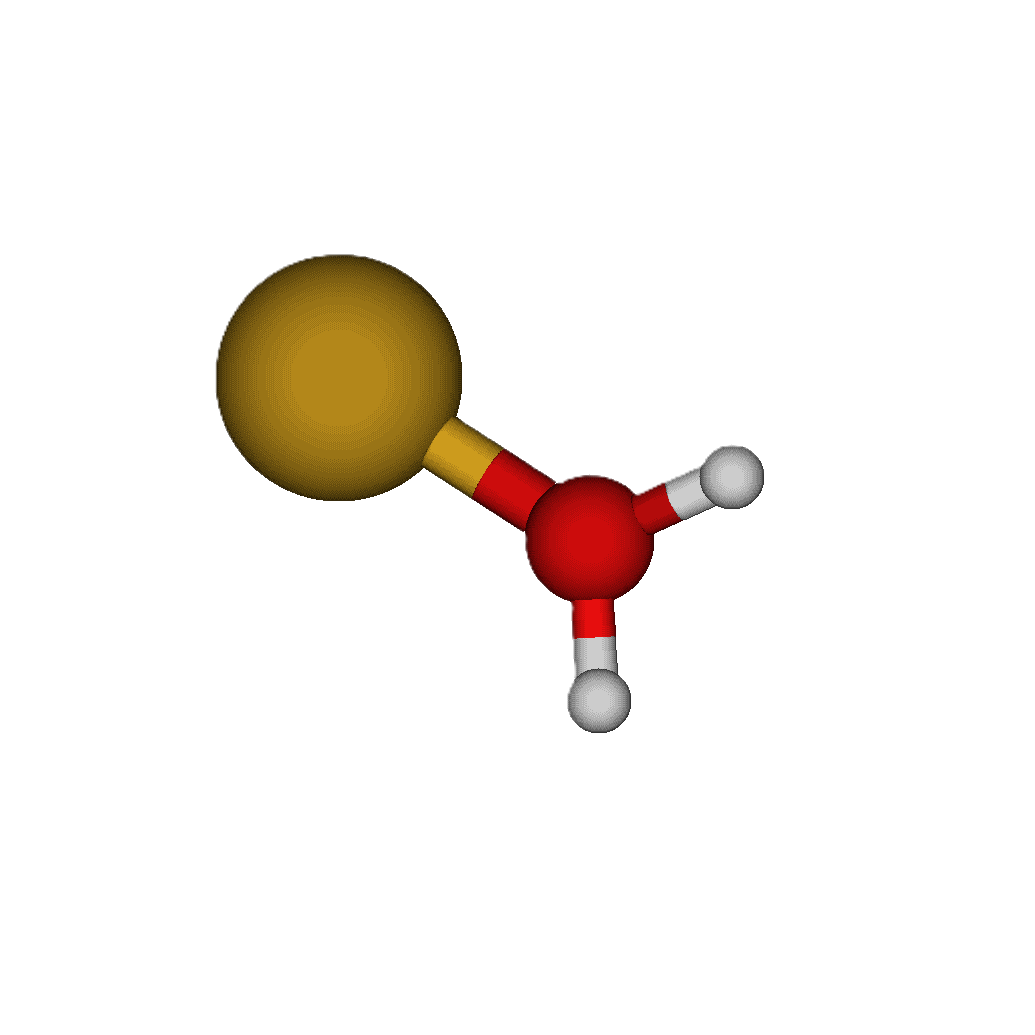
\includegraphics[width=\linewidth]{Imágenes/geometria_opt_n_1.png}
        \text{$n=1$}
    \end{minipage}\hfill
    \begin{minipage}[b]{0.25\textwidth}
        \centering
        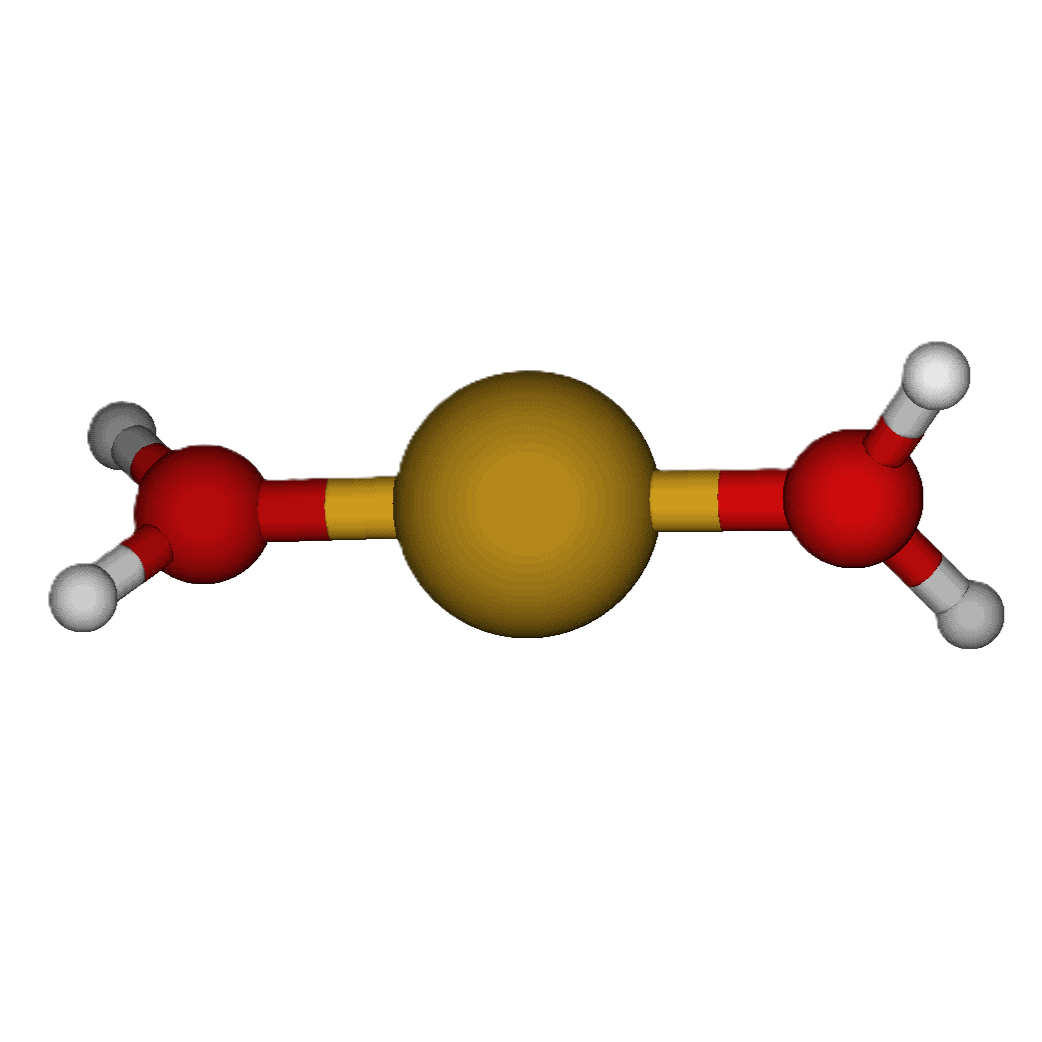
\includegraphics[width=\linewidth]{Imágenes/geometria_opt_n_2.png}
        \text{$n=2$}
    \end{minipage}\hfill
    \begin{minipage}[b]{0.25\textwidth}
        \centering
        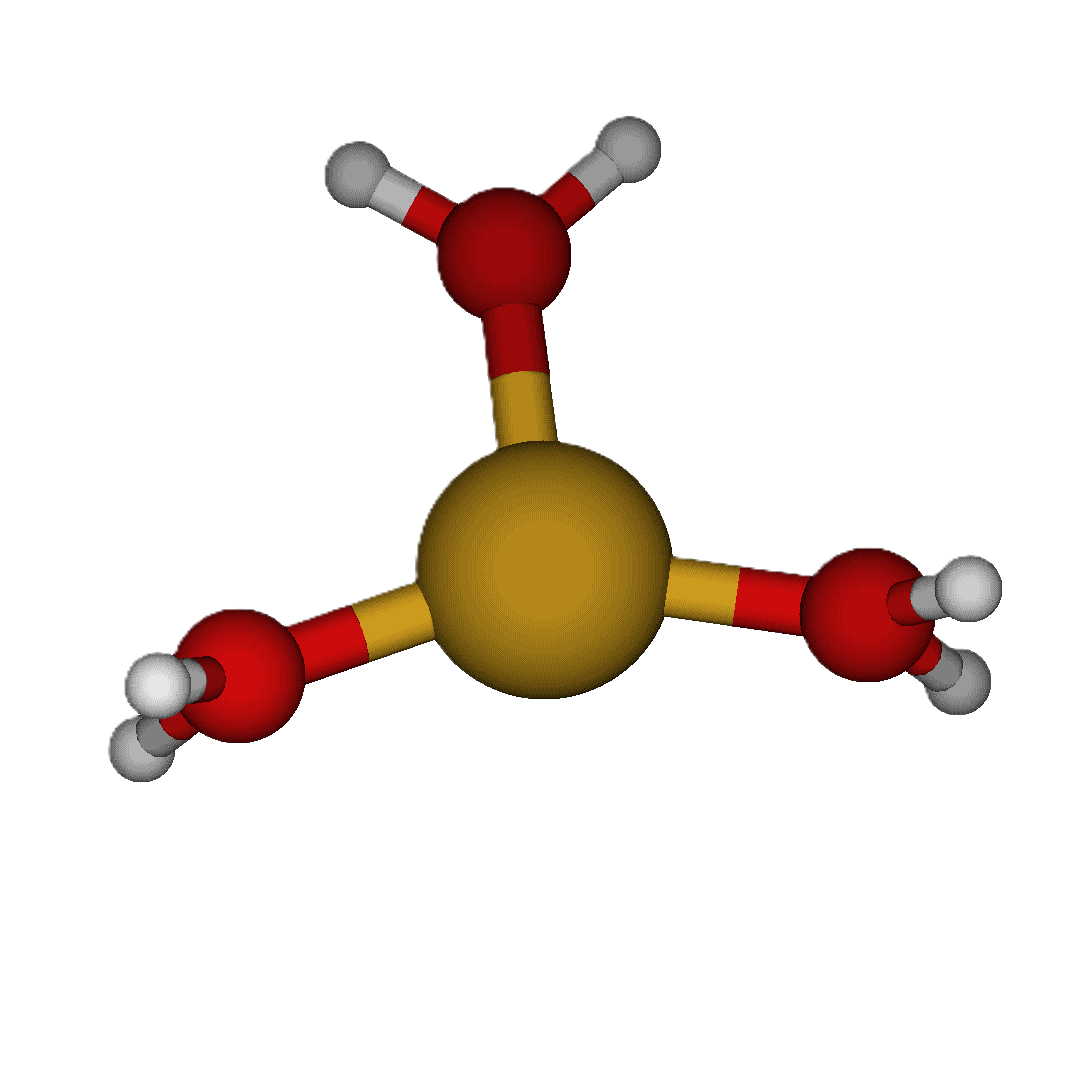
\includegraphics[width=\linewidth]{Imágenes/geometria_opt_n_3.png}
        \text{$n=3$}
    \end{minipage}
    
    \vspace{0.5cm} % Espacio vertical entre filas

    % --- Fila 2 (n=4, 5, 6) ---
    \begin{minipage}[b]{0.25\textwidth}
        \centering
        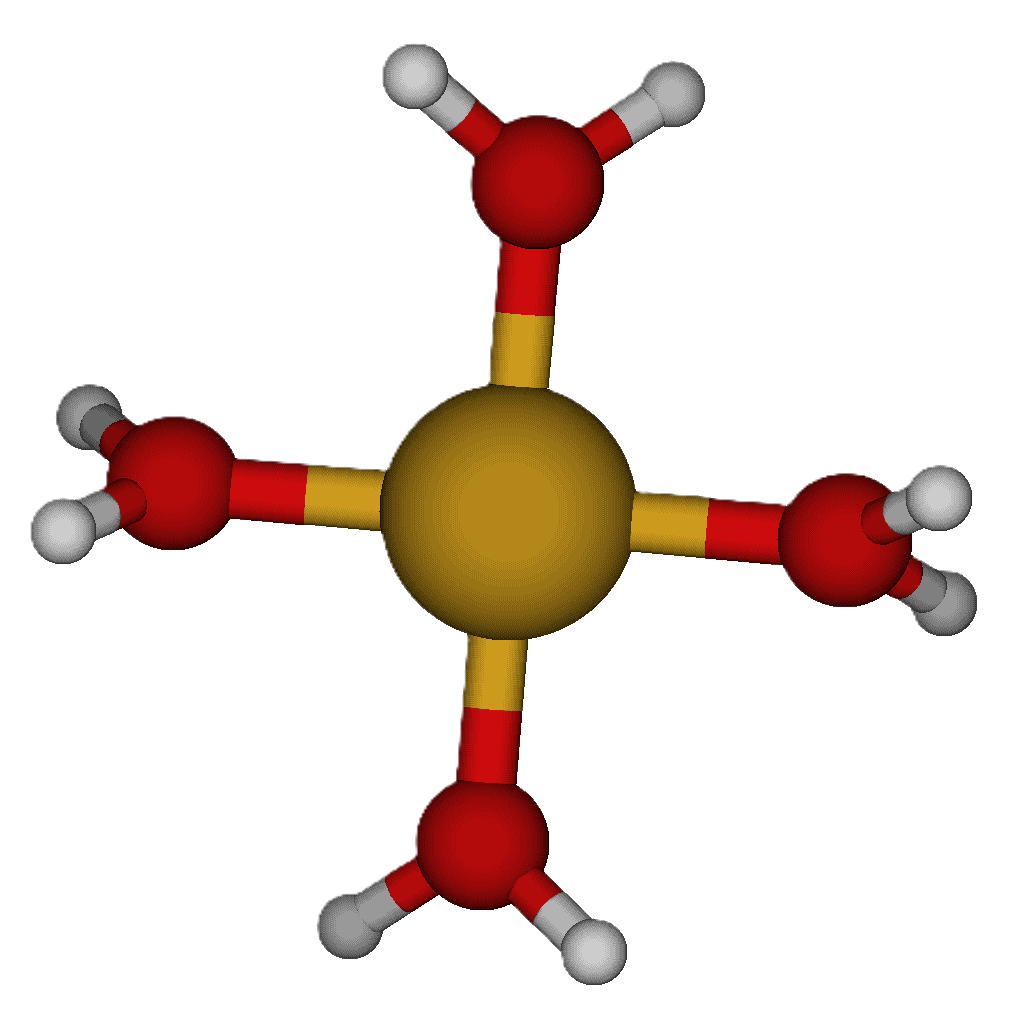
\includegraphics[width=\linewidth]{Imágenes/geometria_opt_n_4.png}
        \text{$n=4$}
    \end{minipage}\hfill
    \begin{minipage}[b]{0.25\textwidth}
        \centering
        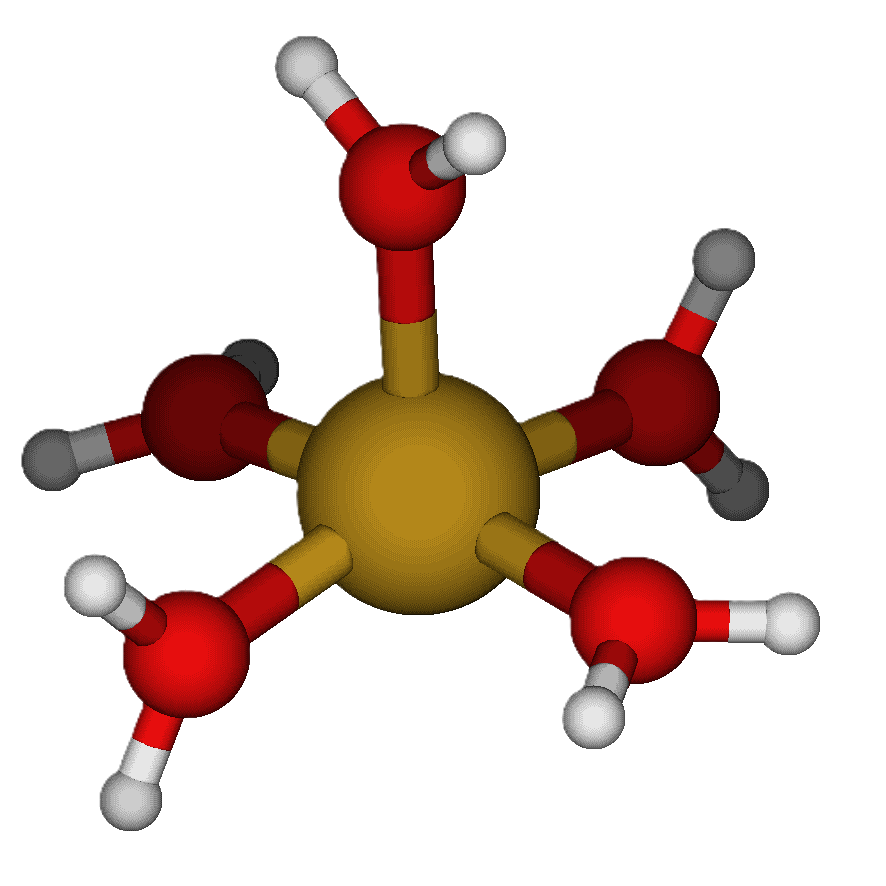
\includegraphics[width=\linewidth]{Imágenes/geometria_opt_n_5.png}
        \text{$n=5$}
    \end{minipage}\hfill
    \begin{minipage}[b]{0.25\textwidth}
        \centering
        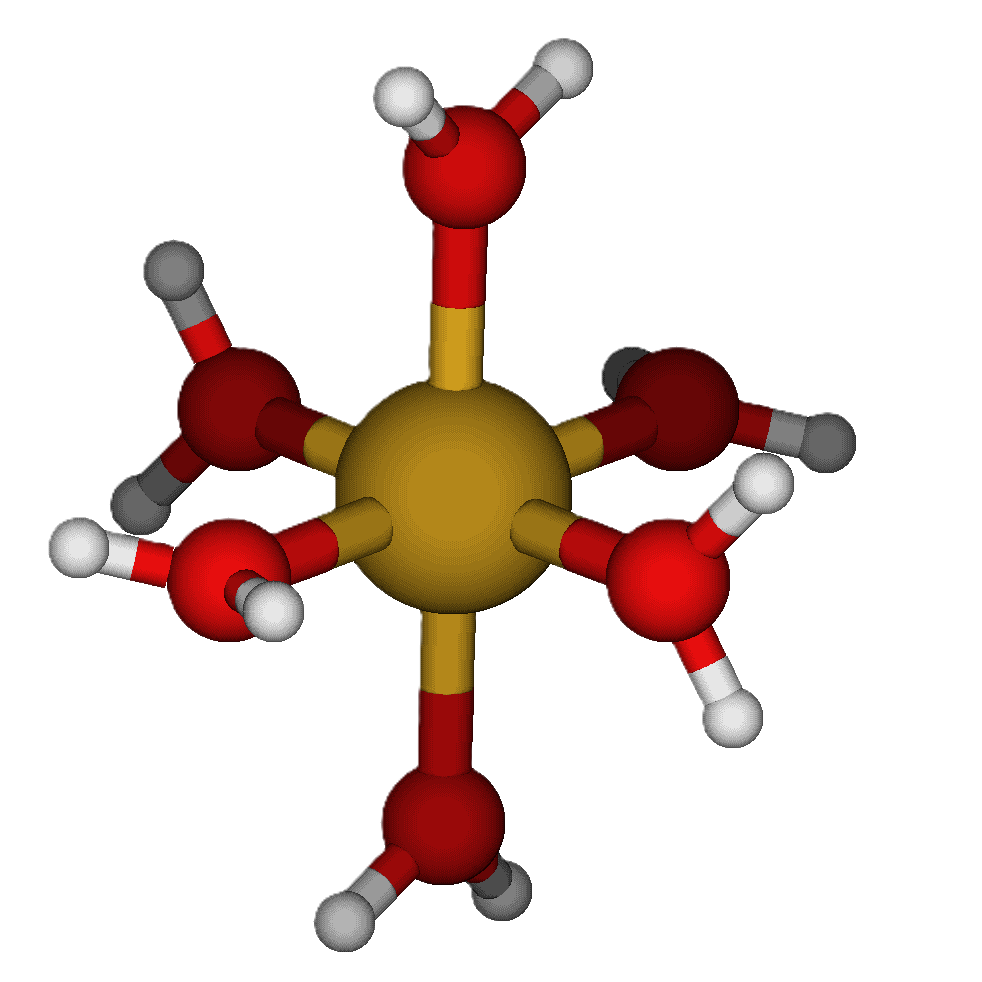
\includegraphics[width=\linewidth]{Imágenes/geometria_opt_n_6.png}
        \text{$n=6$}
    \end{minipage}

    \vspace{0.5cm} % Espacio vertical entre filas
    
    % --- Fila 3 (n=7, 8, 9) ---
    \begin{minipage}[b]{0.25\textwidth}
        \centering
        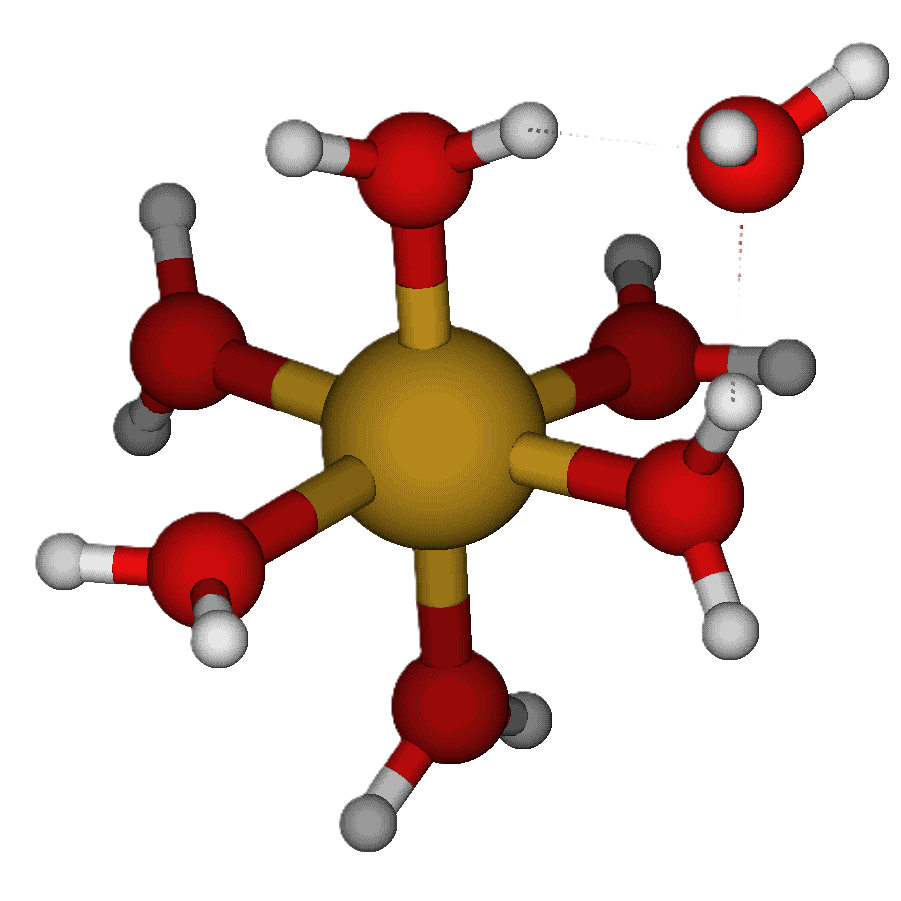
\includegraphics[width=\linewidth]{Imágenes/geometria_opt_n_7.png}
        \text{$n=7$}
    \end{minipage}\hfill
    \begin{minipage}[b]{0.25\textwidth}
        \centering
        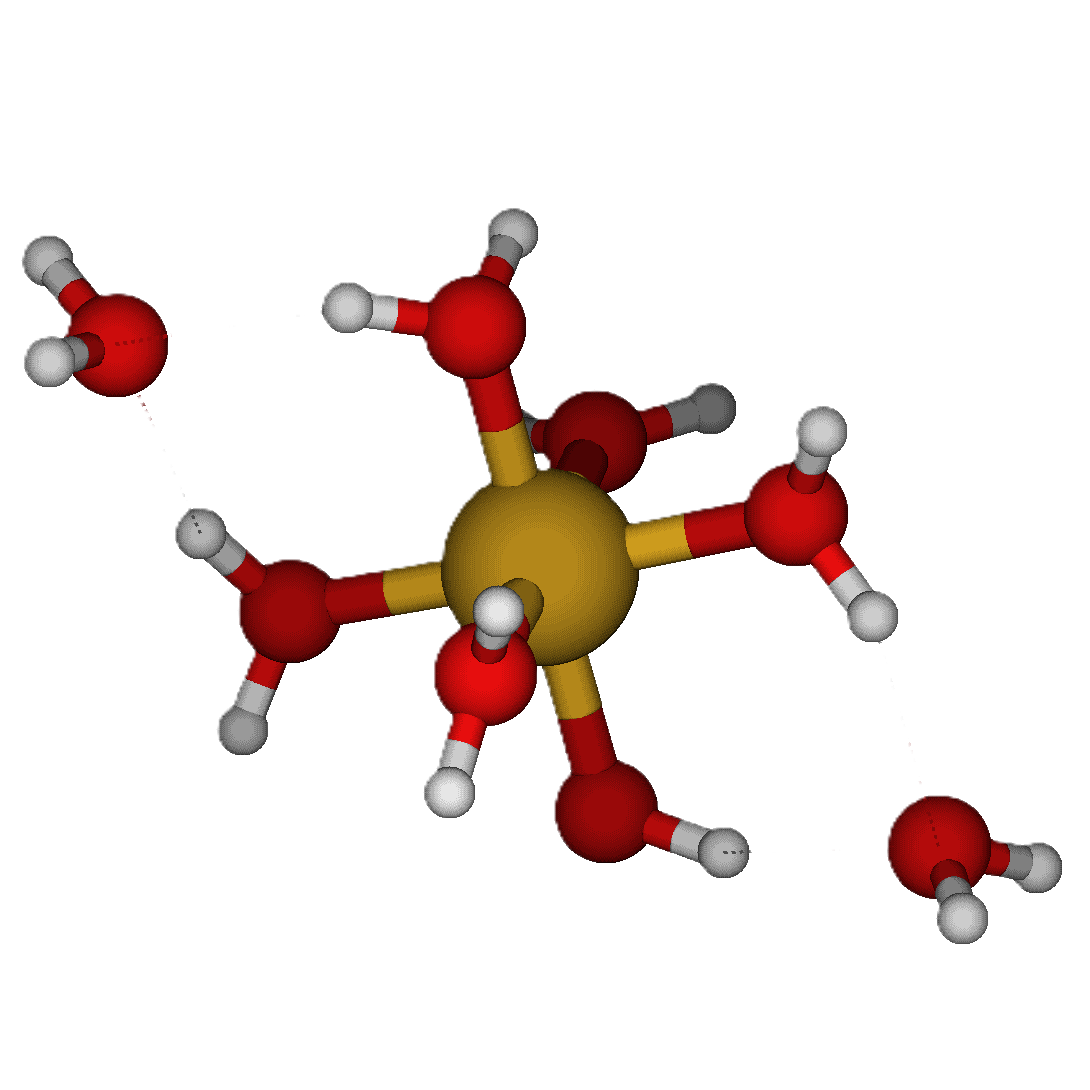
\includegraphics[width=\linewidth]{Imágenes/geometria_opt_n_8.png}
        \text{$n=8$}
    \end{minipage}\hfill
    \begin{minipage}[b]{0.25\textwidth}
        \centering
        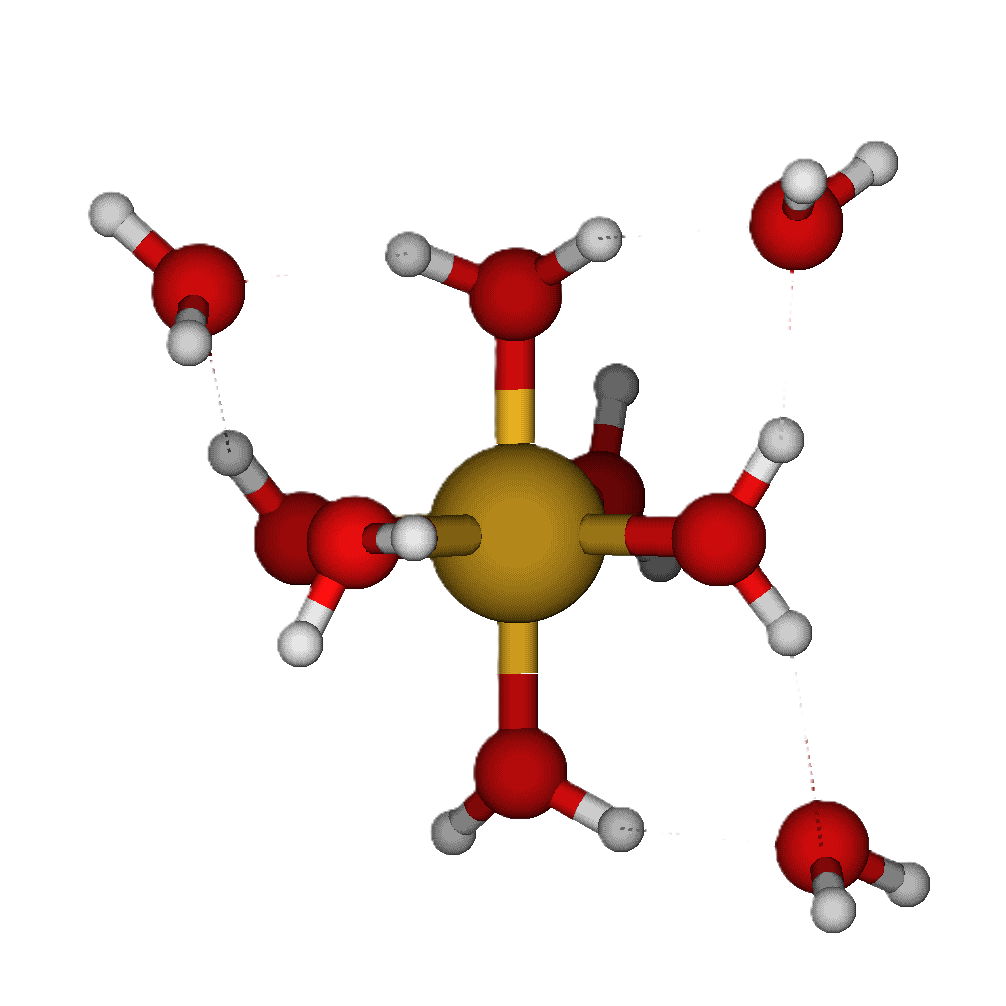
\includegraphics[width=\linewidth]{Imágenes/geometria_opt_n_9.png}
        \text{$n=9$}
    \end{minipage}

    \vspace{0.5cm} % Espacio vertical entre filas

    % --- Fila 4 (n=10, 30, 40) ---
    \begin{minipage}[b]{0.3\textwidth}
        \centering
        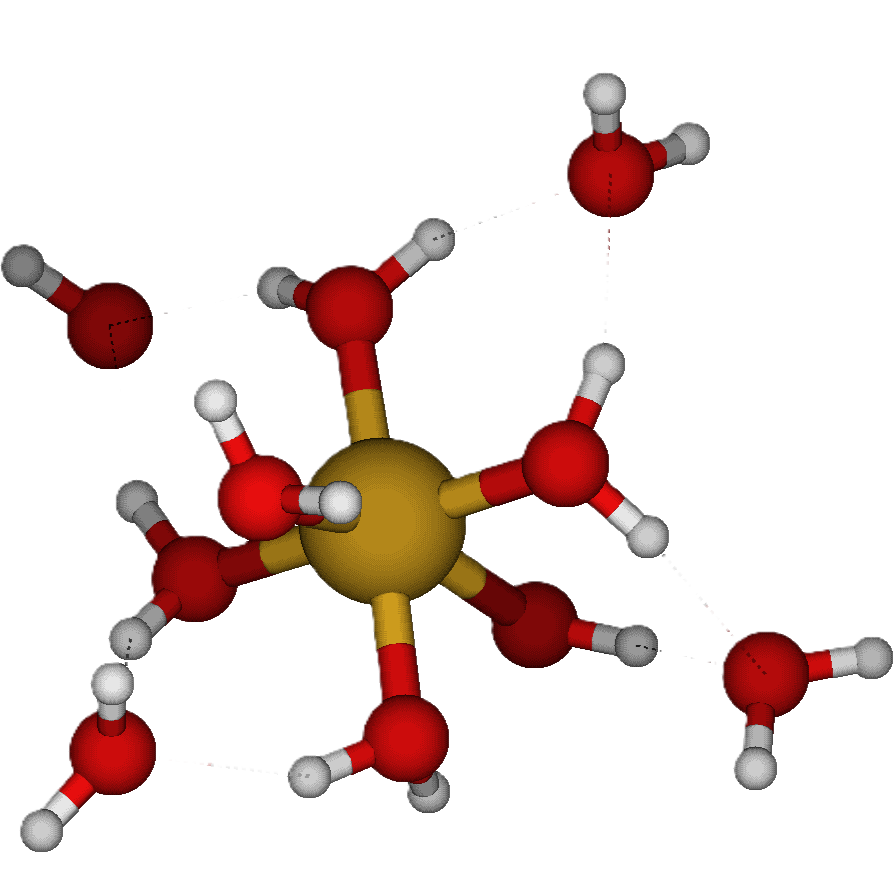
\includegraphics[width=\linewidth]{Imágenes/geometria_opt_n_10.png}
        \text{$n=10$}
    \end{minipage}\hfill
    \begin{minipage}[b]{0.3\textwidth}
        \centering
        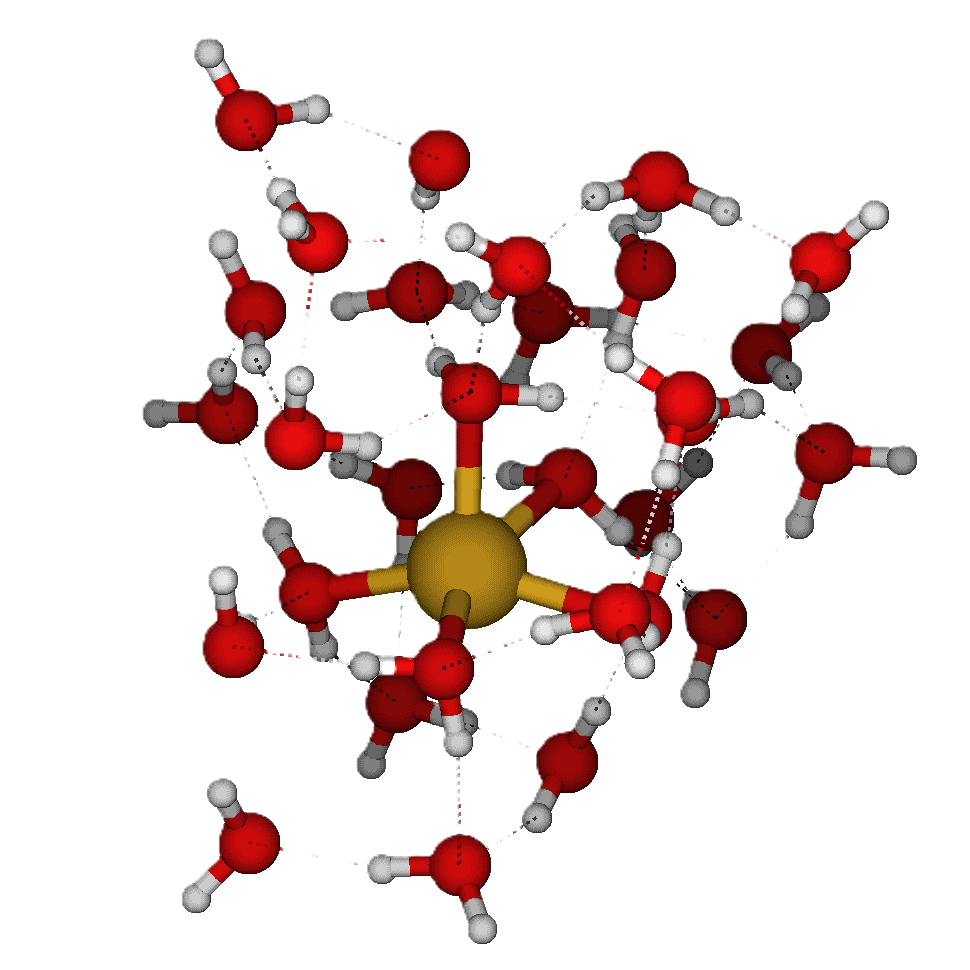
\includegraphics[width=\linewidth]{Imágenes/geometria_opt_n_30.png}
        \text{$n=30$}
    \end{minipage}\hfill
    \begin{minipage}[b]{0.3\textwidth}
        \centering
        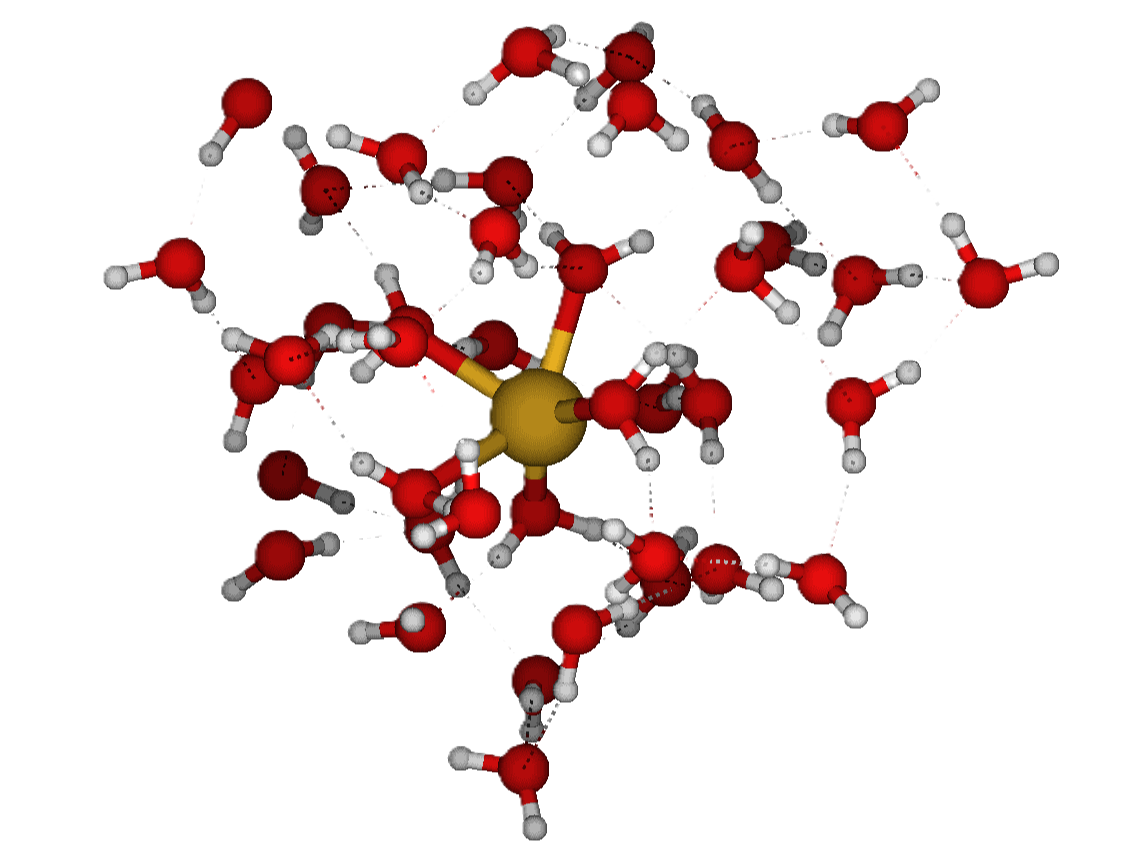
\includegraphics[width=\linewidth]{Imágenes/geometria_opt_n_40.png}
        \text{$n=40$}
    \end{minipage}

\end{figure}


% --- Entorno de Figuras 3x4 ---
\begin{figure}[h!]
    \centering
    \caption{Geometrías optimizadas para los cúmulos \ce{[Cu(CH3OH)_{n}]^{2+}} con $n = 1-10, 30, 40$ en el nivel de teoría 6-31G*.}
    \label{fig:geo_opt_cumulos_m}

    % --- Fila 1 (n=1, 2, 3) ---
    \begin{minipage}[b]{0.25\textwidth}
        \centering
        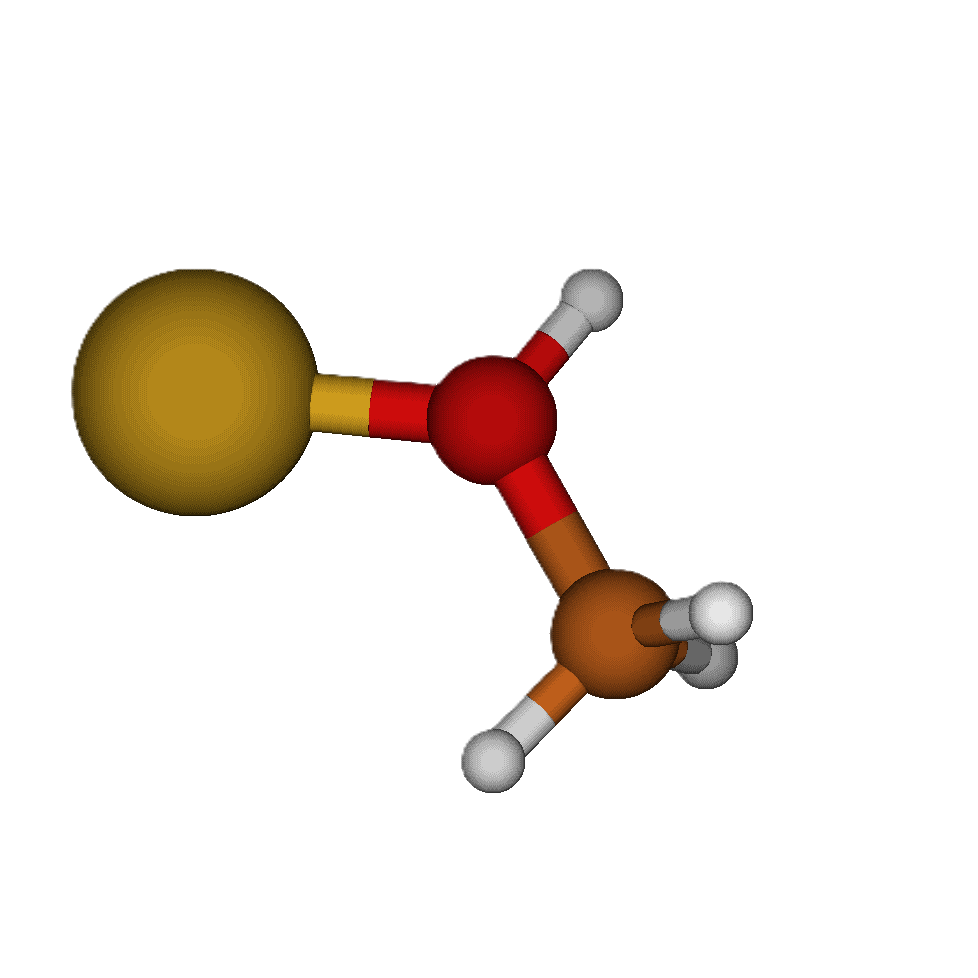
\includegraphics[width=\linewidth]{Imágenes/m_geometria_opt_n_1.png}
        \text{$n=1$}
    \end{minipage}\hfill
    \begin{minipage}[b]{0.25\textwidth}
        \centering
        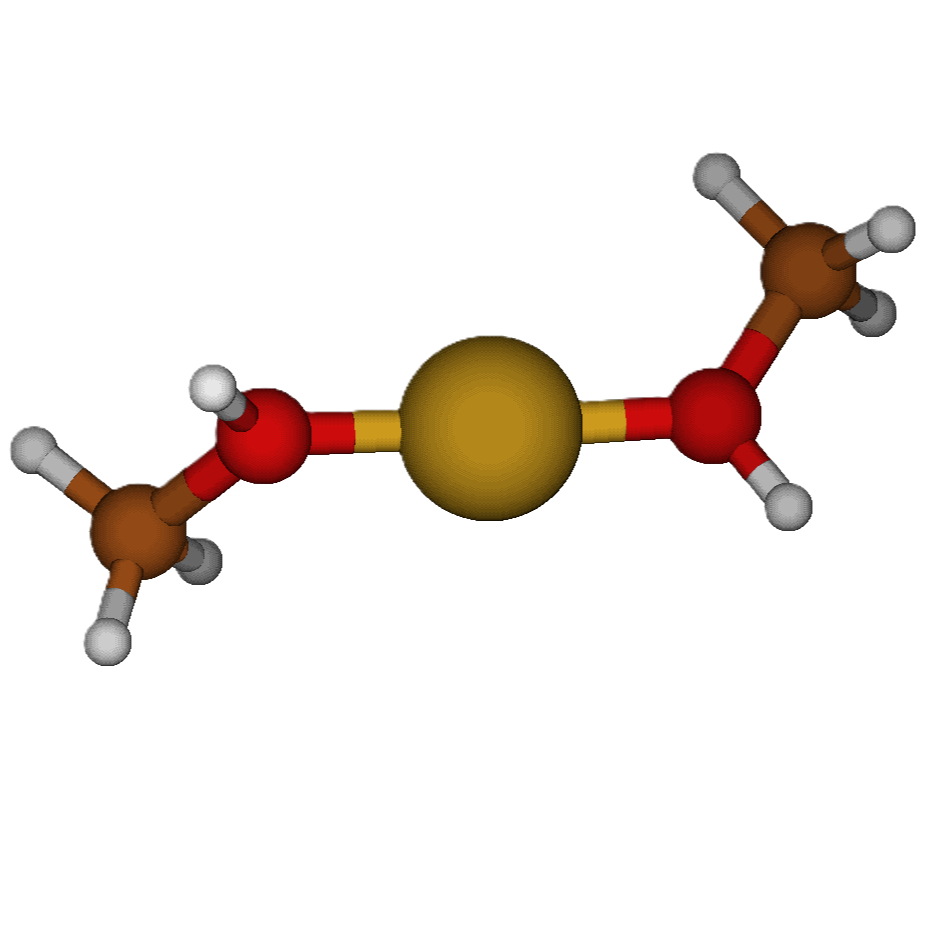
\includegraphics[width=\linewidth]{Imágenes/m_geometria_opt_n_2.png}
        \text{$n=2$}
    \end{minipage}\hfill
    \begin{minipage}[b]{0.25\textwidth}
        \centering
        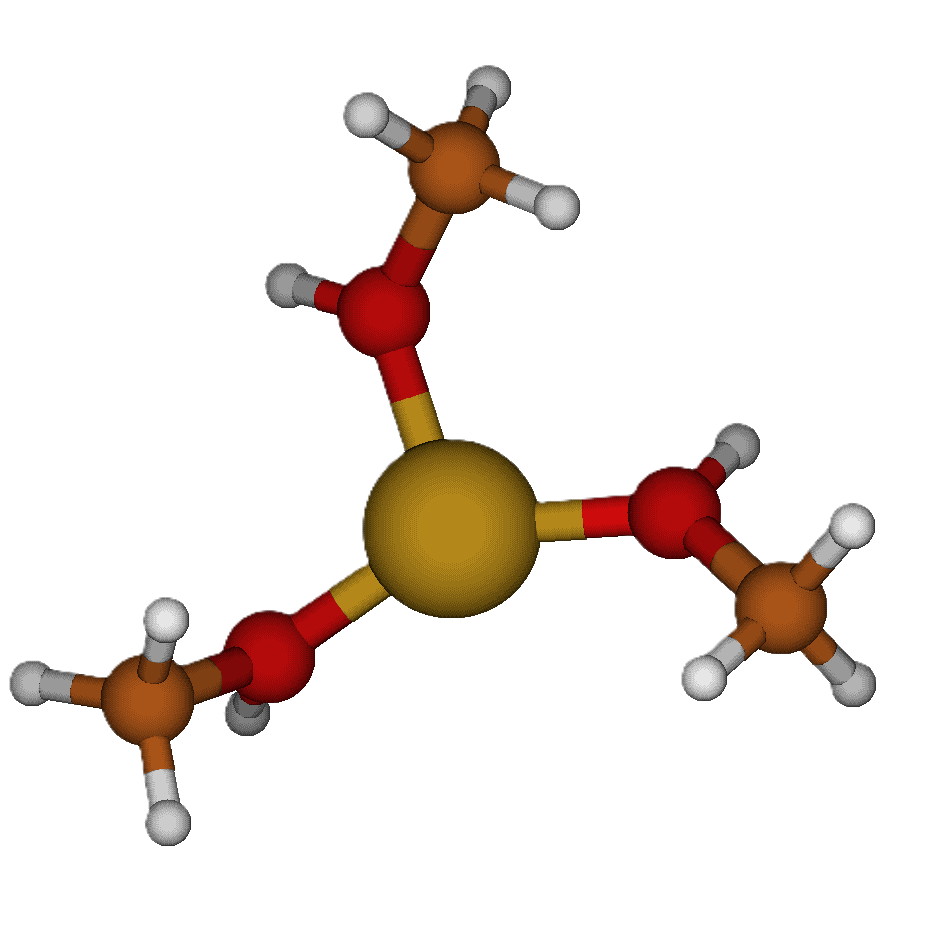
\includegraphics[width=\linewidth]{Imágenes/m_geometria_opt_n_3.png}
        \text{$n=3$}
    \end{minipage}
    
    \vspace{0.5cm} % Espacio vertical entre filas

    % --- Fila 2 (n=4, 5, 6) ---
    \begin{minipage}[b]{0.25\textwidth}
        \centering
        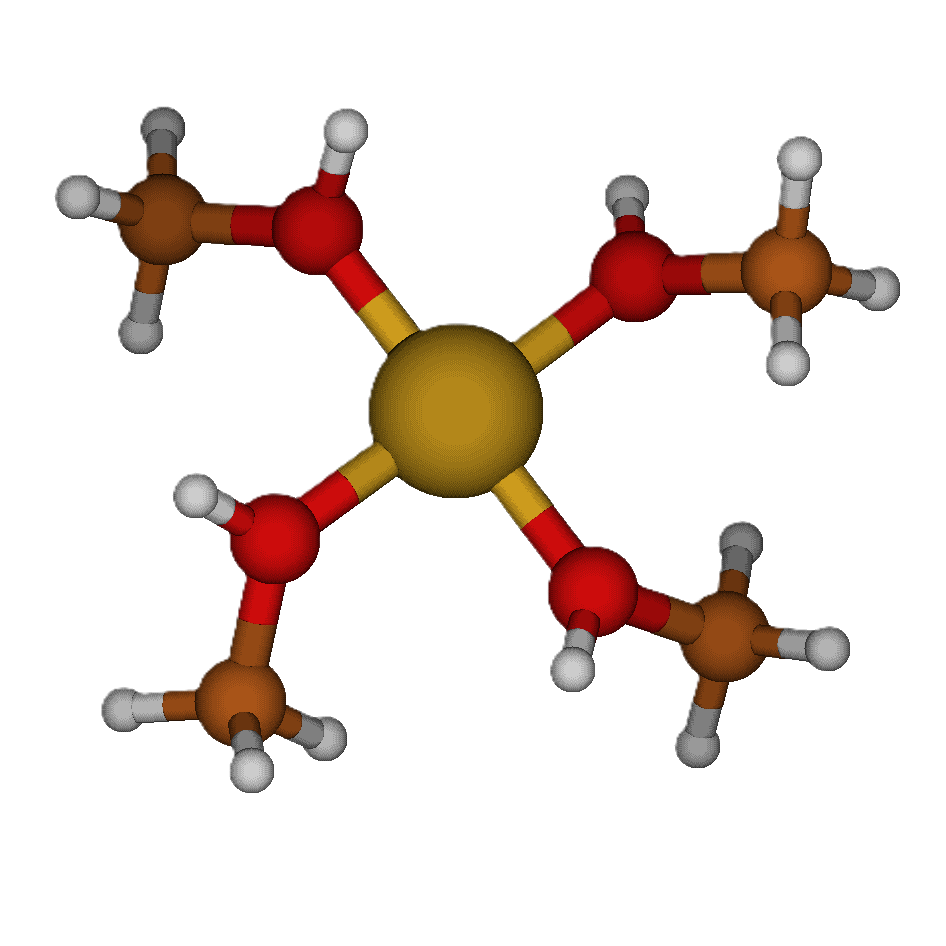
\includegraphics[width=\linewidth]{Imágenes/m_geometria_opt_n_4.png}
        \text{$n=4$}
    \end{minipage}\hfill
    \begin{minipage}[b]{0.25\textwidth}
        \centering
        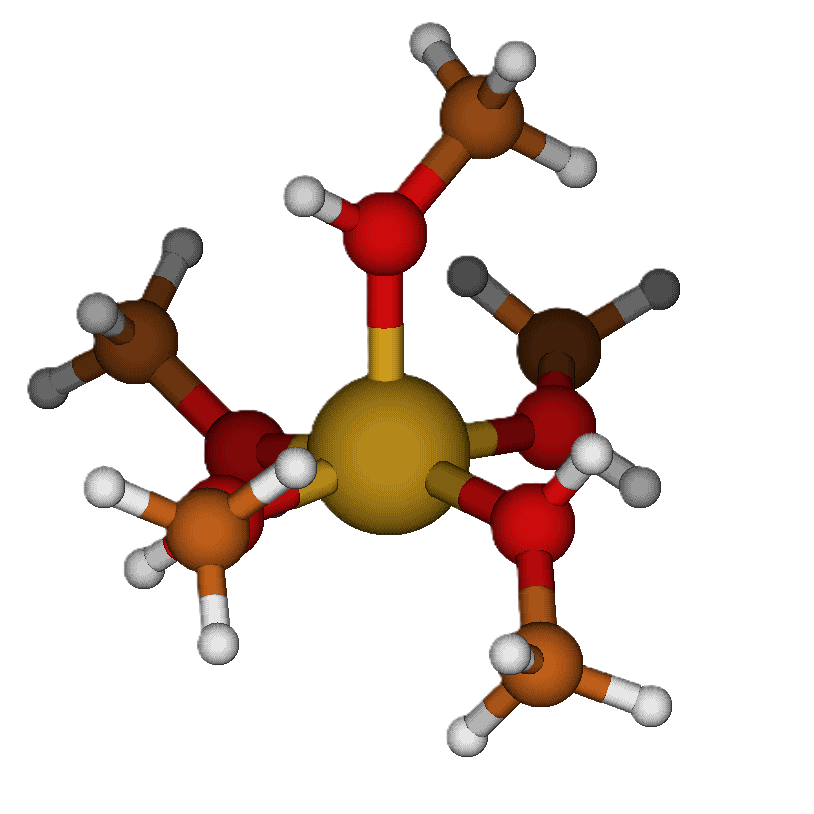
\includegraphics[width=\linewidth]{Imágenes/m_geometria_opt_n_5.png}
        \text{$n=5$}
    \end{minipage}\hfill
    \begin{minipage}[b]{0.25\textwidth}
        \centering
        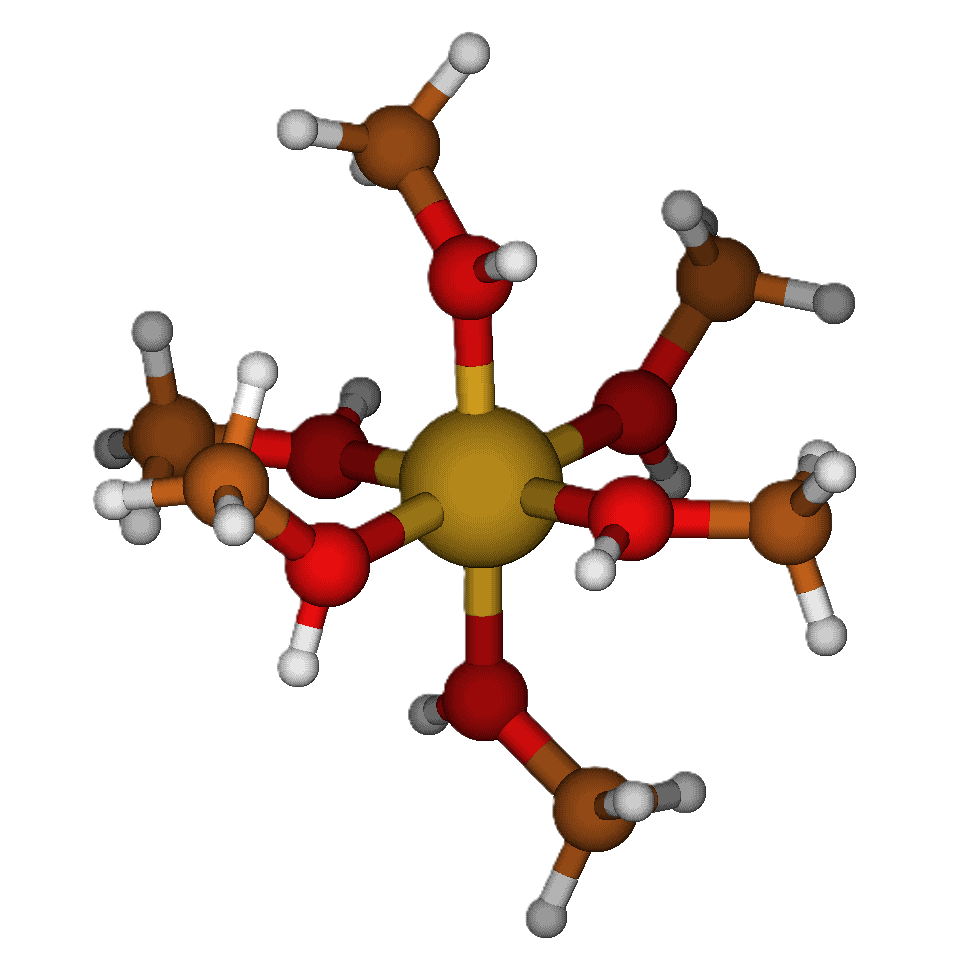
\includegraphics[width=\linewidth]{Imágenes/m_geometria_opt_n_6.png}
        \text{$n=6$}
    \end{minipage}

    \vspace{0.5cm} % Espacio vertical entre filas
    
    % --- Fila 3 (n=7, 8, 9) ---
    \begin{minipage}[b]{0.25\textwidth}
        \centering
        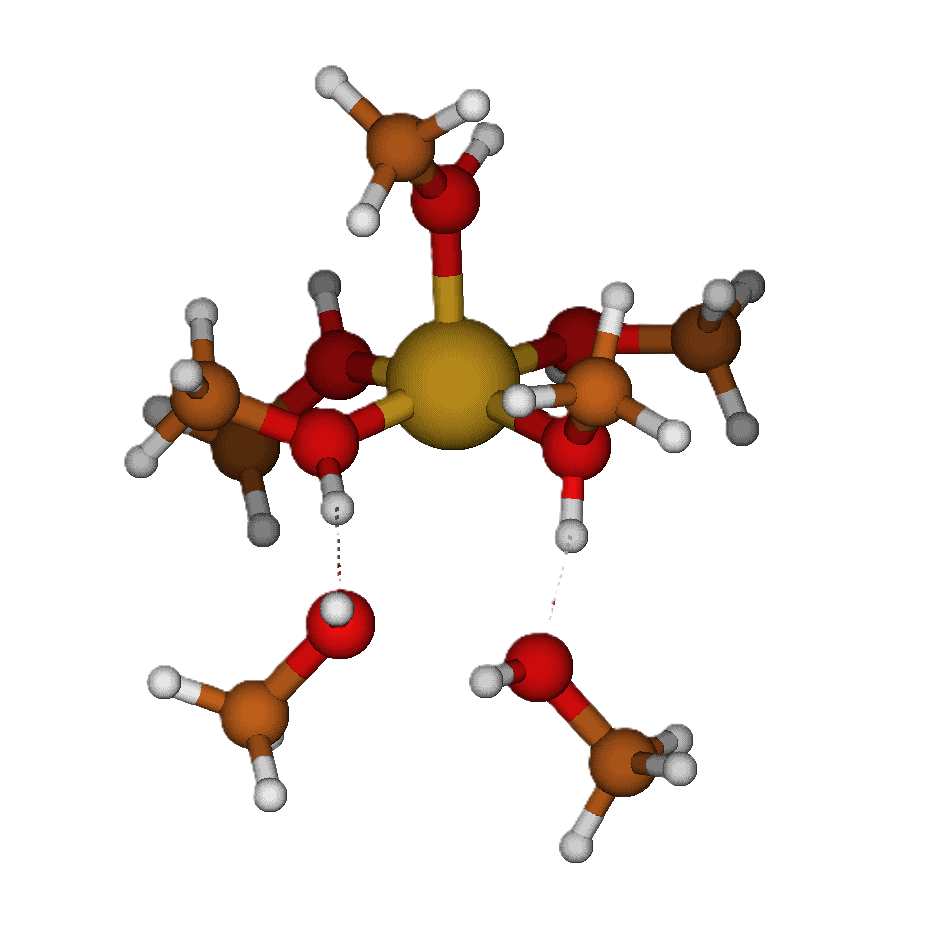
\includegraphics[width=\linewidth]{Imágenes/m_geometria_opt_n_7.png}
        \text{$n=7$}
    \end{minipage}\hfill
    \begin{minipage}[b]{0.25\textwidth}
        \centering
        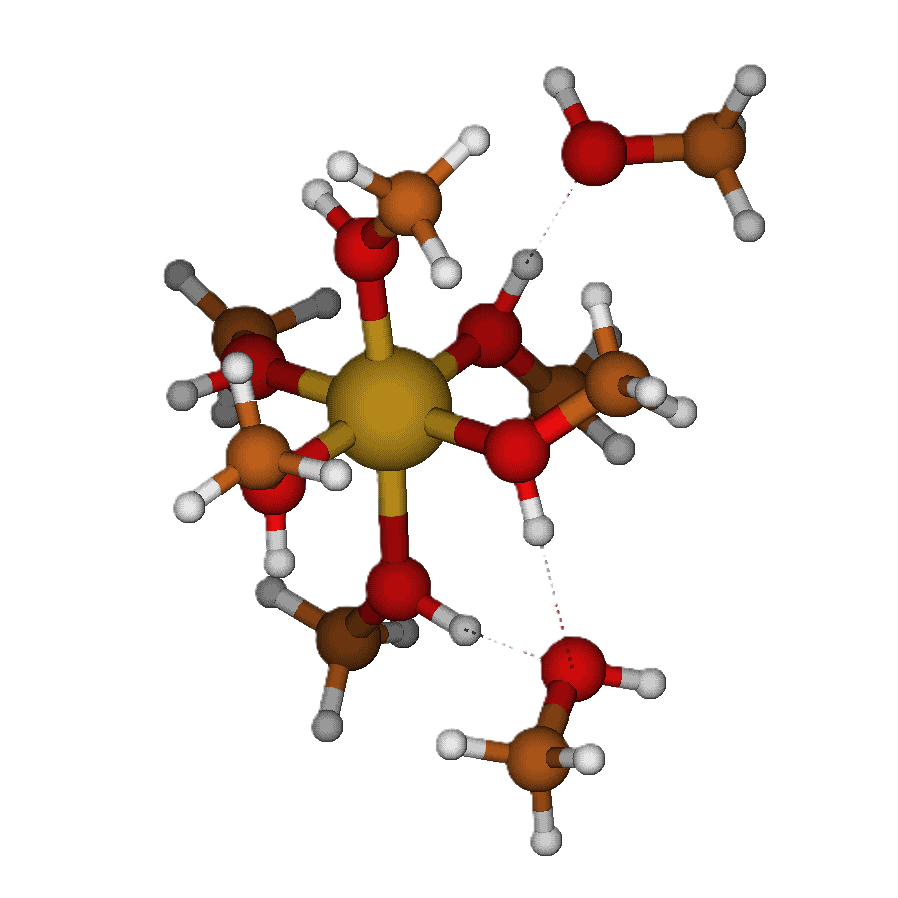
\includegraphics[width=\linewidth]{Imágenes/m_geometria_opt_n_8.png}
        \text{$n=8$}
    \end{minipage}\hfill
    \begin{minipage}[b]{0.25\textwidth}
        \centering
        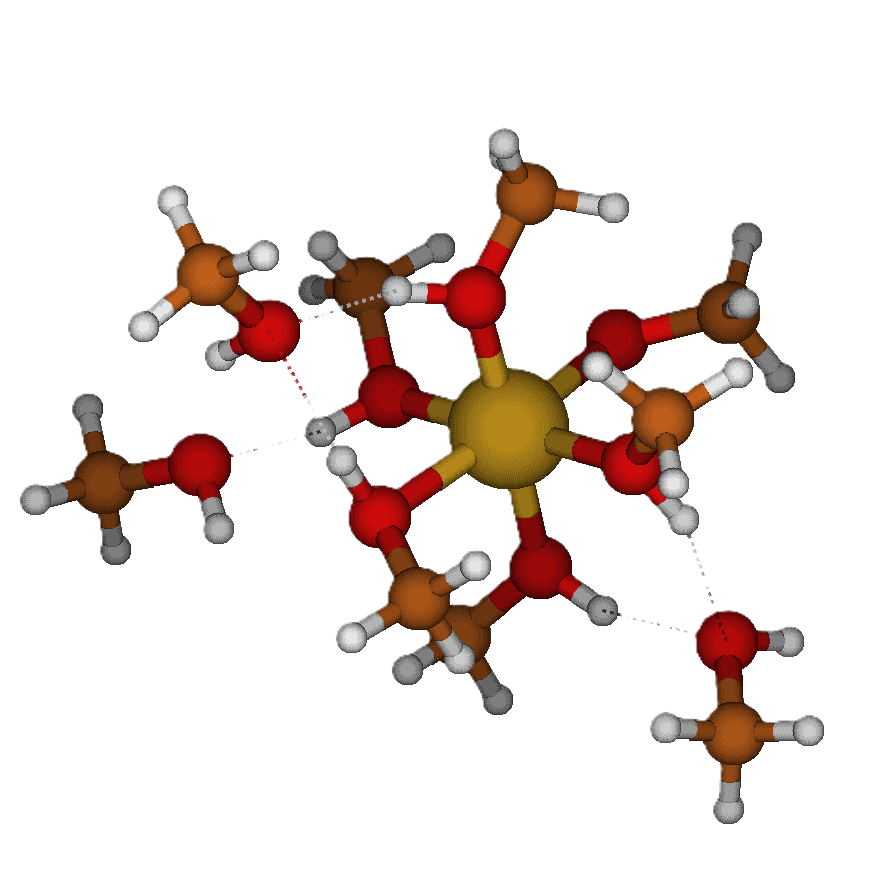
\includegraphics[width=\linewidth]{Imágenes/m_geometria_opt_n_9.png}
        \text{$n=9$}
    \end{minipage}

    \vspace{0.5cm} % Espacio vertical entre filas

    % --- Fila 4 (n=10, 30, 40) ---
    \begin{minipage}[b]{0.3\textwidth}
        \centering
        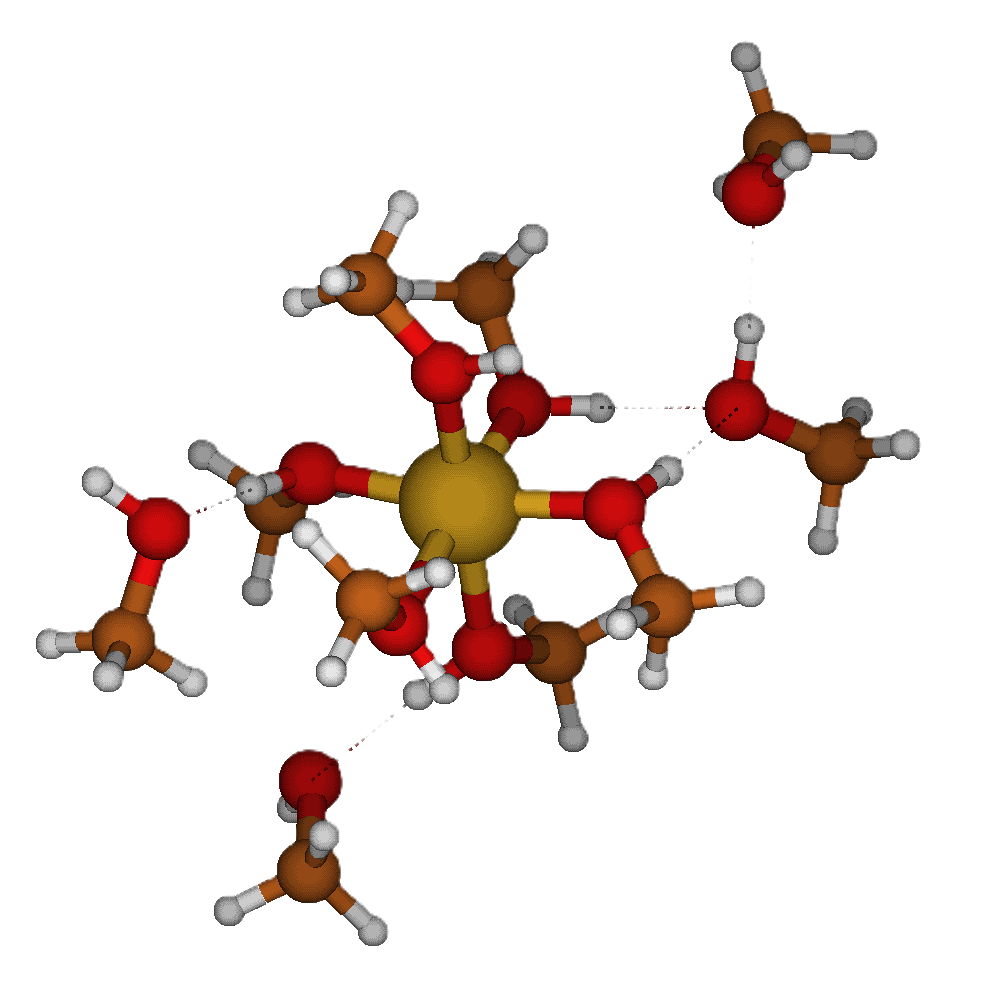
\includegraphics[width=\linewidth]{Imágenes/m_geometria_opt_n_10.png}
        \text{$n=10$}
    \end{minipage}\hfill
    \begin{minipage}[b]{0.3\textwidth}
        \centering
        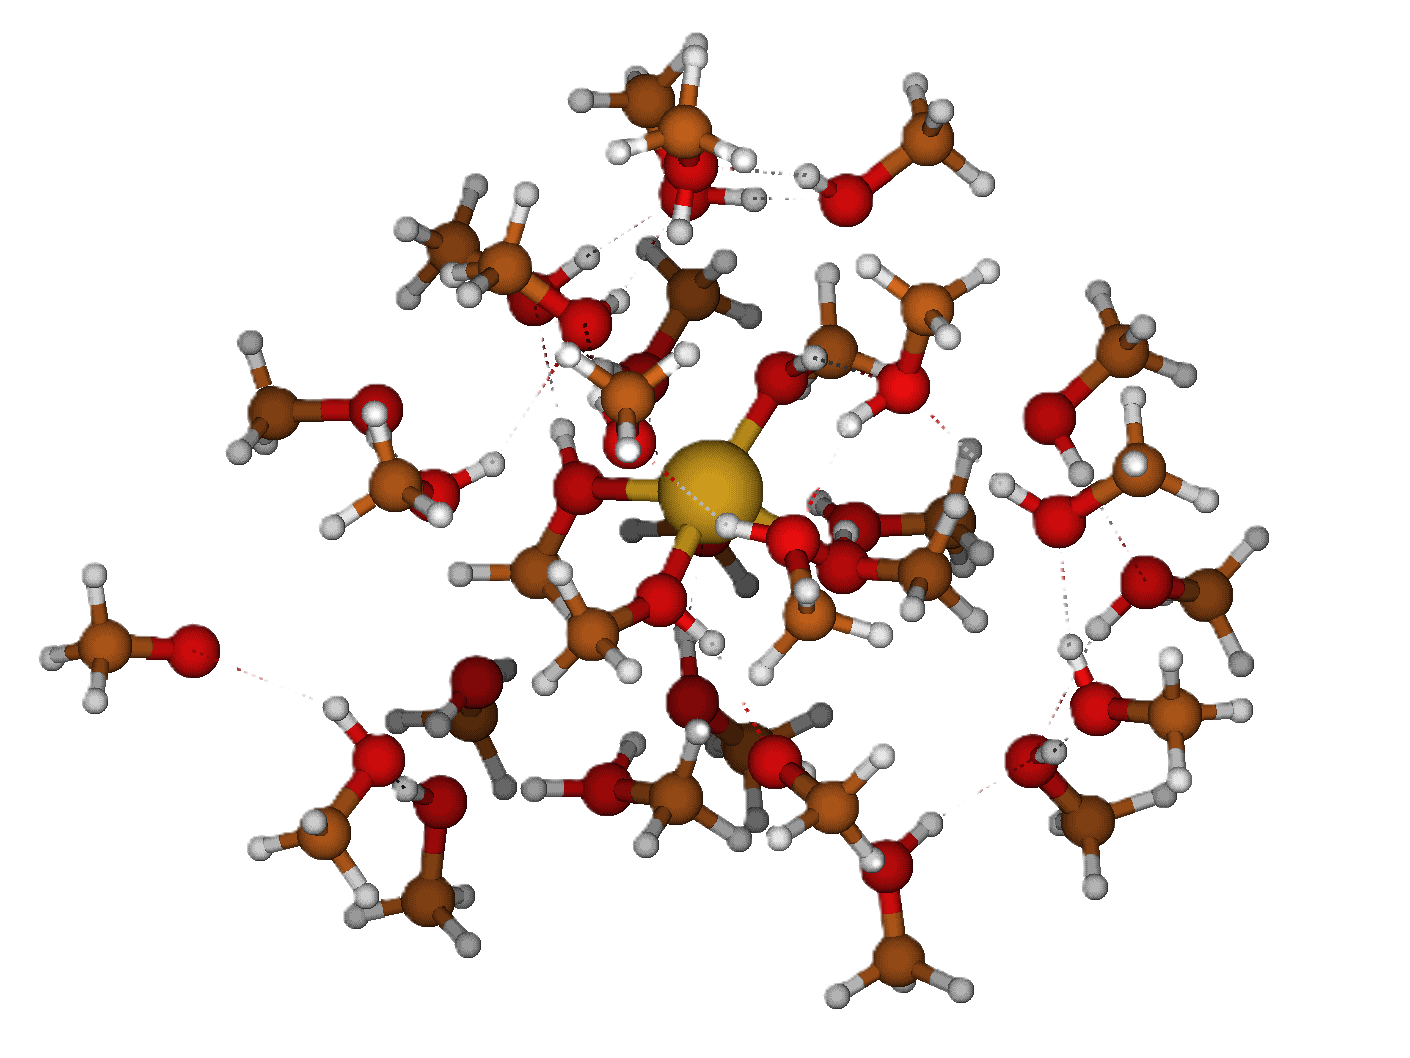
\includegraphics[width=\linewidth]{Imágenes/m_geometria_opt_n_30.png}
        \text{$n=30$}
    \end{minipage}\hfill
    \begin{minipage}[b]{0.3\textwidth}
        \centering
        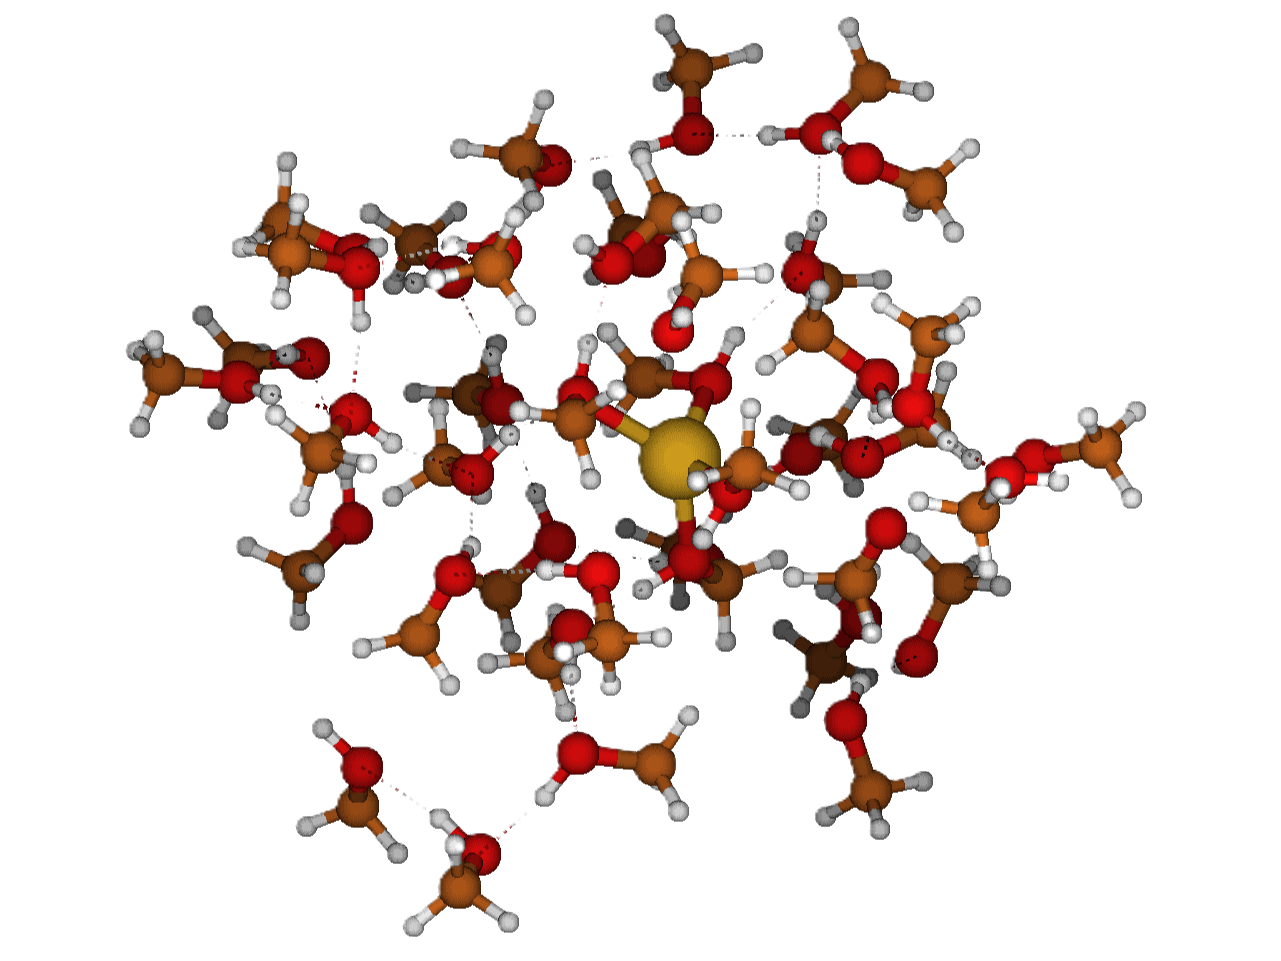
\includegraphics[width=\linewidth]{Imágenes/m_geometria_opt_n_40.png}
        \text{$n=40$}
    \end{minipage}

\end{figure}

\begin{figure}[H]
    \centering
    
    % Gráfica 1 (Agua)
    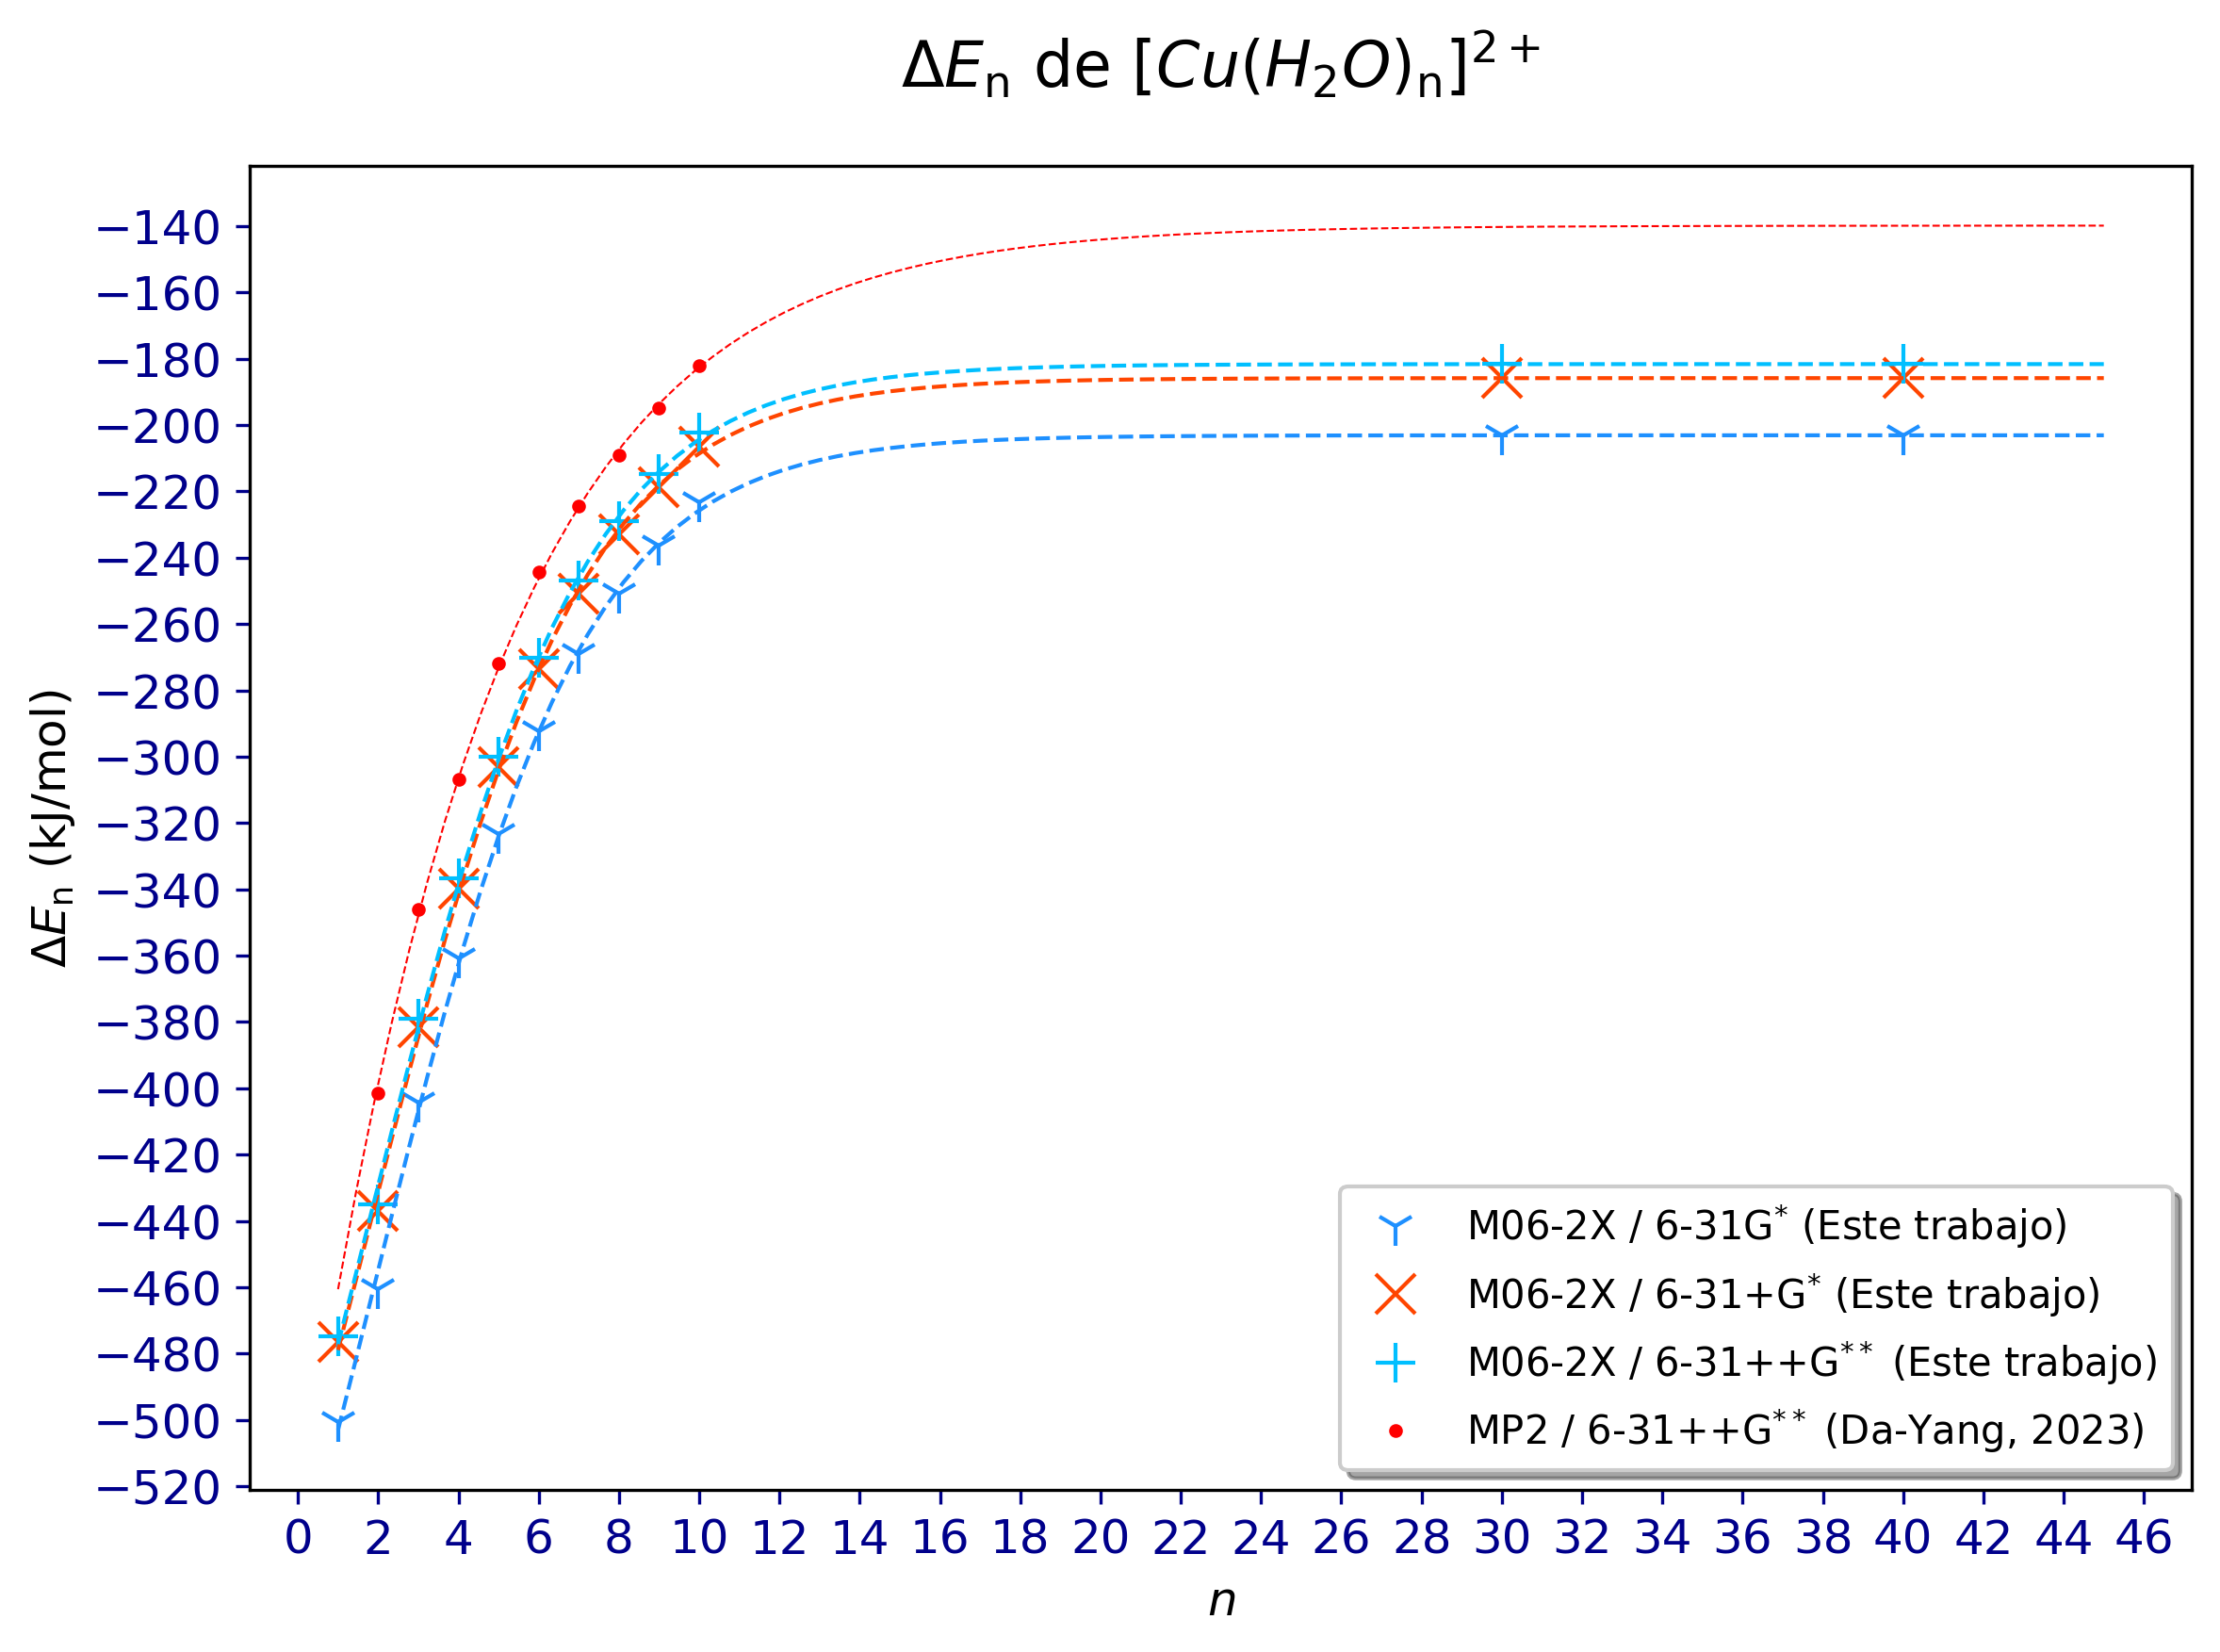
\includegraphics[width=0.85\textwidth]{Imágenes/bases_agua.png}
    
    % Un pequeño espacio vertical entre las gráficas
    \vspace{0.5cm} 
    
    % Gráfica 2 (Metanol)
    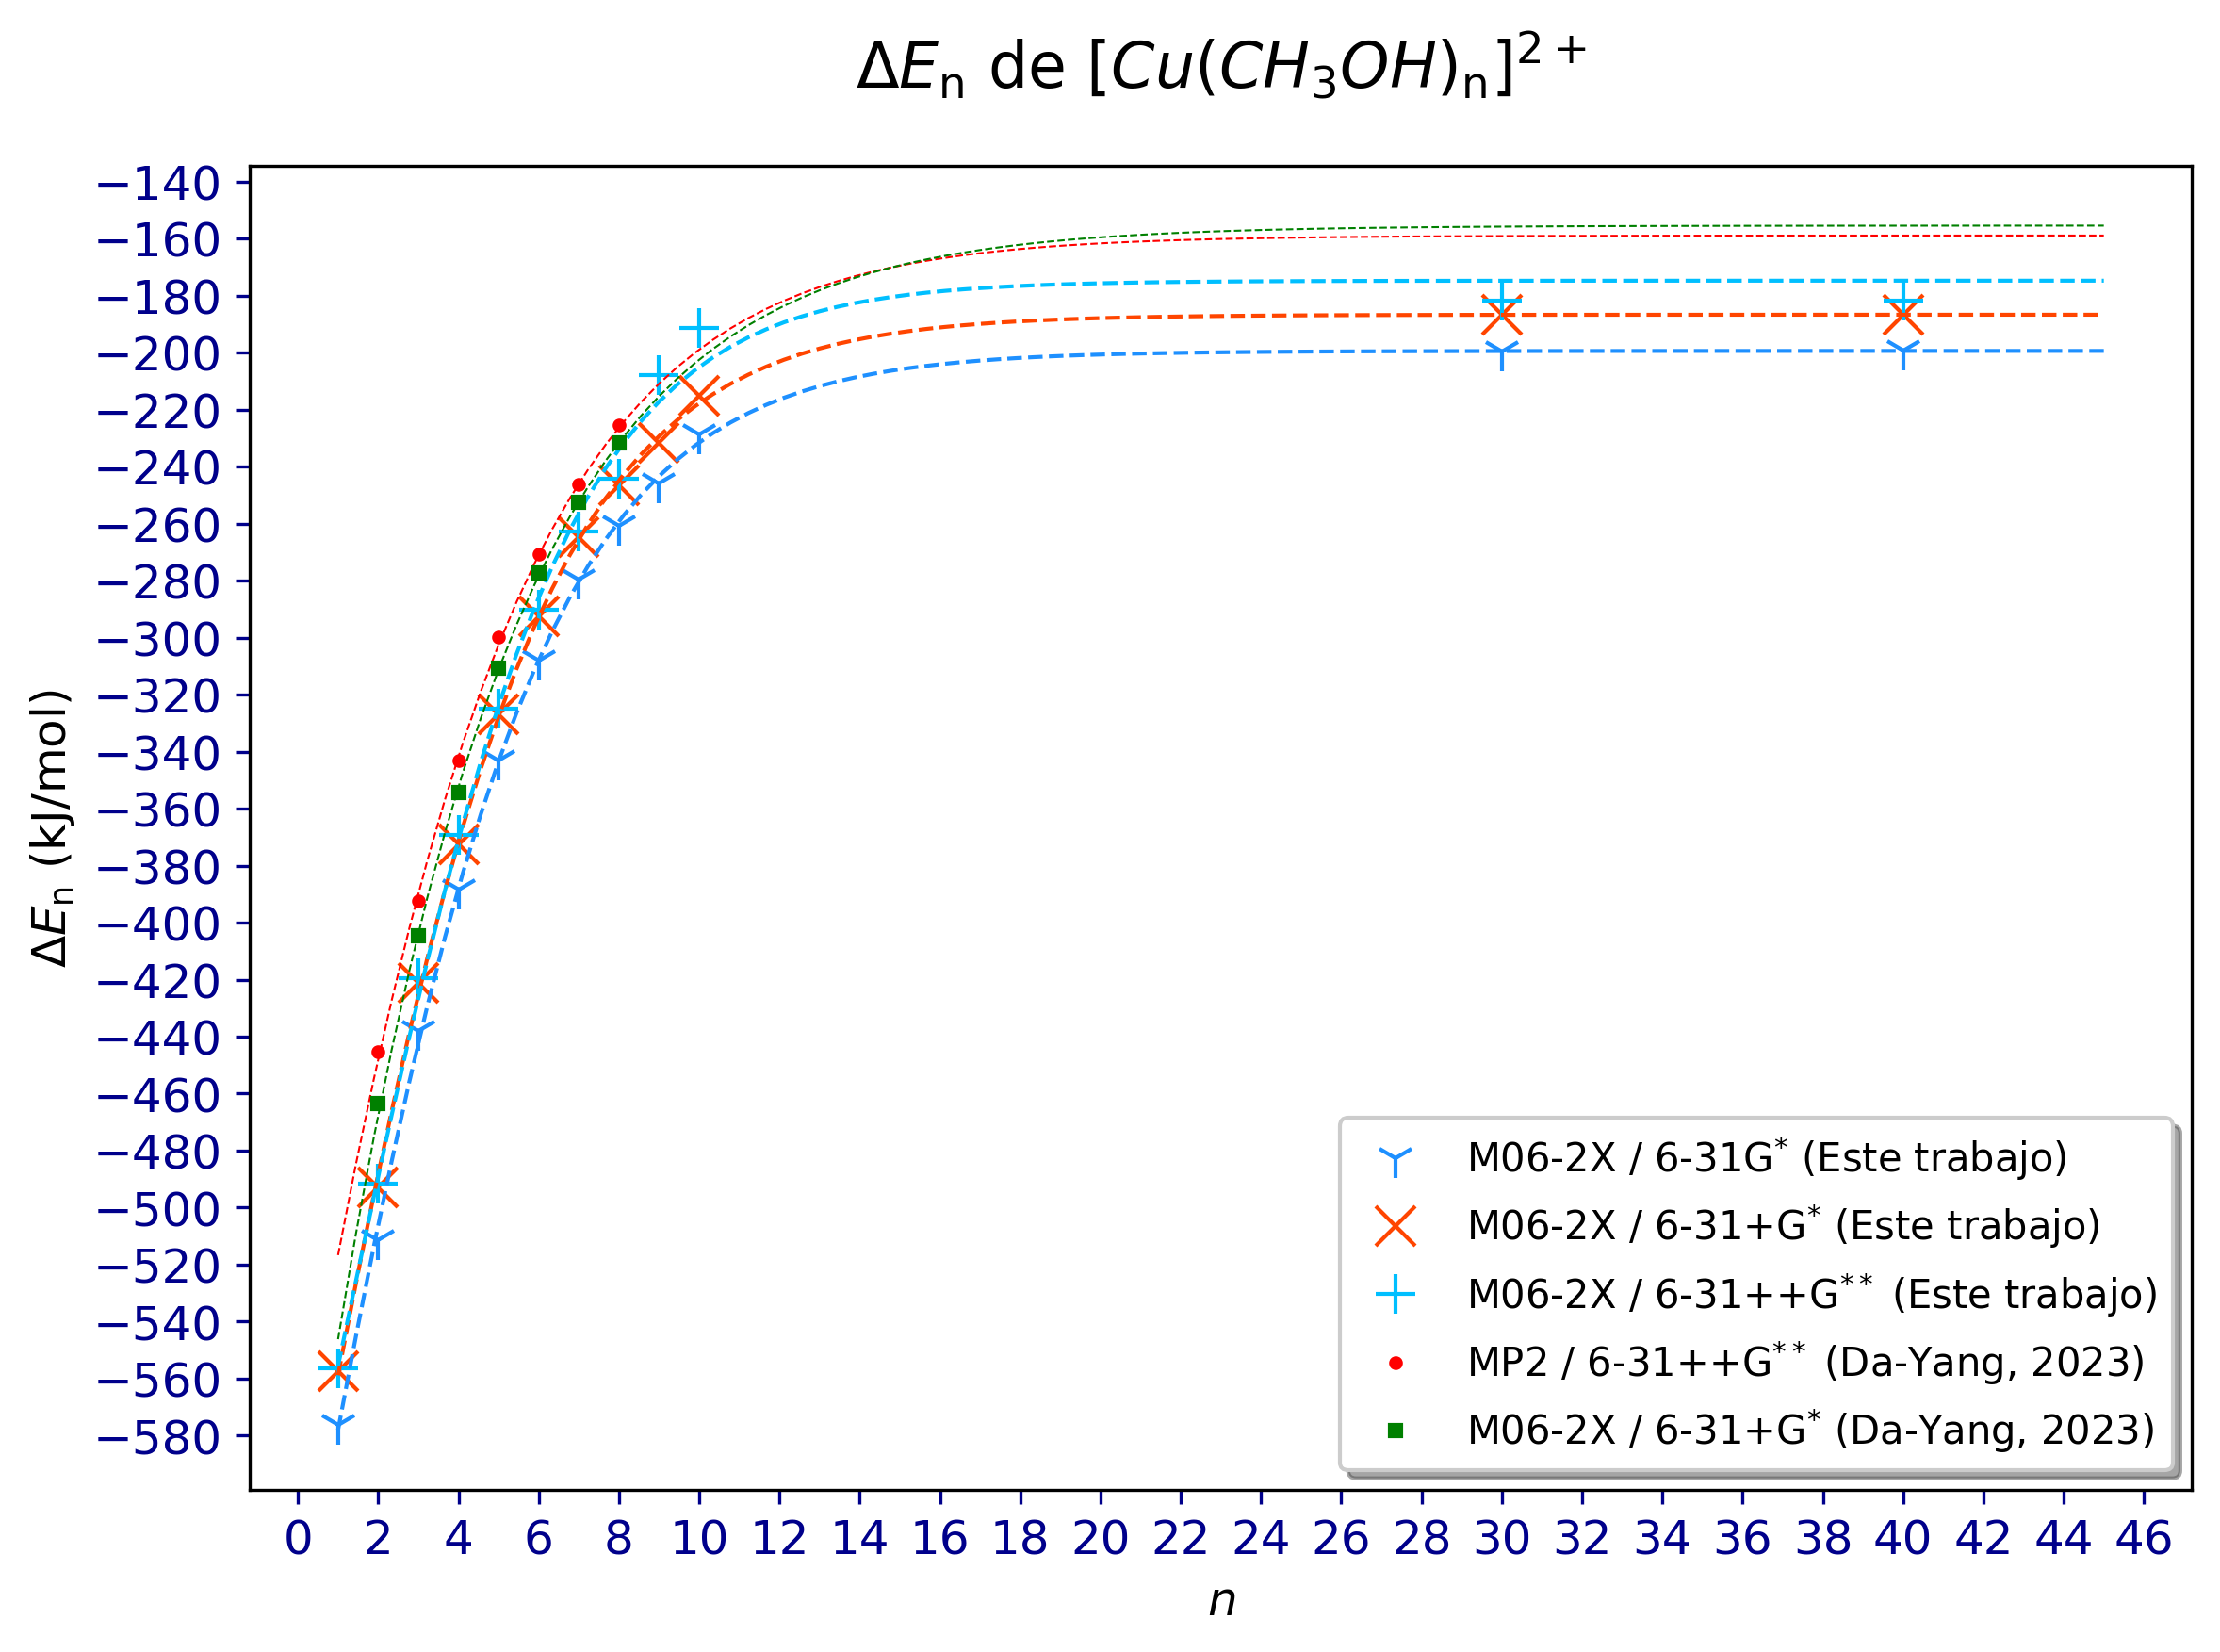
\includegraphics[width=0.85\textwidth]{Imágenes/bases_metanol.png}

    % --- LEYENDA ACTUALIZADA ---
    \caption{Energías de enlace por molécula de solvente calculada para las estructuras de solvatación óptimas de \ce{[Cu(H2O)_{n}]^{2+}} (arriba) y \ce{[Cu(CH3OH)_{n}]^{2+}} (abajo), con $n = 1,\ 2,\ \ldots,\ 10,\ 30,\ 40$, mediante cálculos de optimización con los niveles de teoría 6-31G$^\ast$, 6-31+G$^\ast$ y 6-31++G$^{\ast\ast}$. Resultados obtenidos con MP2 \cite{Me-2022-01} y validación de M06-2X respecto a MP2 \cite{Me-2023-01}.}
    \label{fig:bases}
\end{figure}

Como se observa en la figura \ref{fig:bases}, todos los conjuntos base probados exhiben la misma tendencia en la energía de enlace por molécula de solvente. Para ambos sistemas, $\ce{[Cu(H2O)_{n}]^{2+}}$ (arriba) y $\ce{[Cu(CH3OH)_{n}]^{2+}}$ (abajo), esta tendencia muestra que la energía de enlace es más fuerte para cúmulos pequeños y converge hacia un valor asintótico a medida que $n$ aumenta, alcanzando una saturación aparente para $n \geq 10$.

La observación de esta calibración es que las diferencias cuantitativas entre los tres conjuntos base de la familia Pople (6-31G*, 6-31+G* y 6-31++G**) son mínimas en todo el rango de tamaños de cúmulo. La inclusión de funciones difusas en átomos pesados (6-31+G*) o funciones difusas y de polarización adicionales en los átomos de hidrógeno (6-31++G**) no induce un cambio significativo en la energética de la solvatación para estos sistemas.

Dado que el conjunto base \textbf{6-31G*}, siendo el más eficiente en términos de costo computacional, ofrece resultados virtualmente idénticos a los obtenidos con los conjuntos más grandes y costosos, se seleccionó este conjunto para todas las optimizaciones y simulaciones de dinámica molecular subsecuentes. Esta elección se ve adicionalmente respaldada por la excelente concordancia general de esta familia de métodos con los resultados de referencia de M06-2X \cite{Me-2023-01} y MP2 \cite{Me-2022-01}, también mostrados en la figura.





\section{Simulaciones de Dinámica Molecular}
\label{sec:met_md}

Una vez seleccionado el conjunto base y optimizadas las geometrías de los clústeres de mayor tamaño ($n=40$), se procedió a la fase de producción de la Dinámica Molecular. El objetivo de esta etapa fue generar trayectorias a nivel atomístico para los dos sistemas de interés: \ce{[Cu(H2O)40]^{2+}} y \ce{[Cu(CH3OH)40]^{2+}}, modelados como nanogotas. Todas las simulaciones se realizaron con el módulo \texttt{orca\_md} del paquete ORCA v6.1.

El nivel de teoría empleado fue consistente con la calibración estática. Se utilizó el funcional \textit{meta}-GGA híbrido M06-2X, complementado con la corrección de dispersión D3 de Grimme con amortiguamiento cero (\texttt{D3zero}). Para los átomos de C, H y O se empleó el conjunto base \textbf{6-31G*}. Para el catión \ce{Cu^{2+}}, se utilizó el Potencial de Núcleo Efectivo (ECP) de 10 electrones (N\_core 10) y la base GTO asociada.

Las simulaciones se llevaron a cabo en el ensamble canónico (NVT). Los parámetros clave que definieron la propagación de la dinámica y el control termodinámico se resumen en la Tabla \ref{tab:md_params}.

% --- Tabla de Parámetros de MD ---
\begin{table}[H]
    \centering
    \caption{Parámetros de simulación empleados para cada Dinámica Molecular.}
    \label{tab:md_params}
    \begin{tabular}{ll}
        \hline
        \textbf{Parámetro} & \textbf{Value} \\ \hline
        Ensamble & NVT (Canónico) \\
        Temperatura objetivo ($T$) & 300 K \\
        Asignación de velocidad inicial & Maxwell-Boltzmann (a 300 K) \\
        Termostato & Cadena de Nosé-Hoover (NHC) \\
        \quad - Longitud de la cadena & 4 \\
        \quad - Integrador & Yoshida-7 \\
        Paso de tiempo ($\Delta t$) & 0.5 fs \\
        Tiempo total de producción & 30 ps \\
        Pasos totales de producción & 60,000 \\
        Frecuencia de muestreo & 1 paso (0.5 fs) \\ \hline
    \end{tabular}
\end{table}
% --- Fin de la Tabla ---

El flujo de cálculo seguido en las simulaciones de MD mediante un diagrama de flujo se ilustra en la Figura \ref{fig:metodologia}

% --- Mover este bloque antes de \section{Simulaciones de Dinámica Molecular} ---

\begin{figure}[H] % El [H] fuerza la posición exacta
    \centering
    \caption{Diagrama general de cálculo. Los dos principales bucles son los referentes a el método de campo autoconsistente (SCF) y al principal de la dinámica molecular.}
    \label{fig:metodologia}
    \vspace{0.5cm}
    
    % Rotamos el diagrama 90 grados para mantener el formato horizontal
    \rotatebox{90}{
        \begin{tikzpicture}[
        scale=0.4, transform shape,
        font=\large\sffamily,
        node distance = 8mm and 15mm, % Distancia vertical y horizontal
        block/.style = {rectangle, draw, text centered, rounded corners,
                        minimum height=2.2cm, align=center},
        diamond_dec/.style = {diamond, draw, text centered, aspect=2,
                              inner sep=1pt, text width=2.5cm},
        line/.style = {-{Stealth[length=2.5mm]}}
        ]

        % --- Fila Superior ---
        \node[block] (cond) {\textbf{Inicialización}  \\ $R^{N}(t=0)$};
        \node[block, right=of cond] (opt_structure) {\textbf{Optimizar estructura} \\ {\text{Minimizar energía}} \\ $R^{N}_{min}(0)$};
        \node[block, right=of opt_structure](init_vel) {\textbf{Velocidades} \\ \textbf{iniciales} \\$V^{N}(t=0)$};
        \node[block, right=of init_vel] (t_step) { \textbf{Bucle SCF} \\ $t^{(n)}$};



        % --- Fila Intermedia (Bucle SCF) ---
        \node[block, right=3cm of t_step] (propose_rho){ \textbf{Proponer} \\$\rho^{(n)}(r)$};
        \node[block, below=2.3cm of propose_rho] (build_h) {\textbf{Construir hamiltoniano} \\ $H^{(n)}_{KS} = -\frac{1}{2} \nabla^2 + V_{\text{ext}} + V_H^{(n)} + V_{xc}^{(n)}$};
        \node[block, right=of build_h] (solve_ks) {\textbf{Resolver ecuaciones} \\ \textbf{de Kohn-Sham} \\ $H^{(n)}_{KS} \psi_i = \epsilon_i\psi_i$};
        \node[block, right=of solve_ks] (calc_rho) {\textbf{Calcular nueva densidad} \\ $\rho^{(n+1)}(r) = \sum_{i=1}^{N_{occ}} |\psi_i(r)|^2$};
        \node[diamond_dec, above=1.8cm of calc_rho, xshift=0cm, minimum width=6cm, minimum height=2.5cm] (scf_check) {  \textbf{¿Converge?}  };
        \node[block, right=of scf_check, xshift=1cm] (forces) {\textbf{Calcular energía y fuerzas} \\ $E[\rho] = T_s[\rho] + V_H[\rho] + E_{xc}[\rho] + V_{ext}[\rho]$ \\ $F_I = -\nabla_{R_I} E[\rho]$};

        % --- Fila Inferior (Bucle de Dinámica) ---
        % ***** LÍNEA MODIFICADA AQUÍ *****
        \node[block, below=5.5cm of forces] (vel_update) {\textbf{Actualizar velocidades} \\ \text{Integración + Nosé-Hoover} \\  $V^{N}(t + \Delta t)$ , $T \approx 300\,\text{K}$ };
        \node[block, left=11.5cm of vel_update] (pos_update) {\textbf{Actualizar posiciones} \\ \text{Integración} \\ $R^{N}( t + \Delta t)$};

        % --- Inicio y Fin ---
        \node[block, left=of cond] (start) {Inicio};
        \node[diamond_dec, left=11.5cm of pos_update] (main_loop_check) {¿$t < 20\,\text{ps}$?};
        \node[block, left=of main_loop_check] (analysis) {\textbf{Análisis}};
        \node[block, left=of analysis] (end) {Fin};

        % --- Conexiones con Flechas ---
        % Flujo principal
        \draw[line] (start) -- (cond);
        \draw[line] (cond) -- (opt_structure);
        \draw[line] (opt_structure) -- (init_vel);
        \draw[line] (init_vel) -- (t_step);
        \draw[line] (t_step) -- (propose_rho);

        % Bucle SCF
        \draw[line] (propose_rho) -- (build_h);
        \draw[line] (build_h) -- (solve_ks);
        \draw[line] (solve_ks) -- (calc_rho);
        \draw[line] (calc_rho) -- (scf_check);
        \draw[line] (scf_check) -- node[above] {Sí} (forces);
        \draw[line] (scf_check.west) -- ++(-0.5,0) -| node[below, pos=0.25] {$\rho^{(n)}(r) = \rho^{(n+1)}(r)$}  node[above, pos=0.25] {No} (propose_rho.east);

        % Bucle de Dinámica
        \draw[line] (forces) -- (vel_update);
        \draw[line] (vel_update) -- (pos_update);
        \draw[line] (pos_update) -- (main_loop_check);

        % Bucle principal y final
        \draw[line] (main_loop_check.north) -| node[left, pos=0.8] {Si} (t_step.south);
        \draw[line] (main_loop_check) -- node[below, pos=0.5] {No} (analysis);
        \draw[line] (analysis) -- (end);

        

        \end{tikzpicture}
    }
\end{figure}


\section{Función de Distribución Radial}

%%%%%%%%%%%%%%%%%%%%%%%%%%%%
La Función de Distribución Radial (RDF, por sus siglas en inglés) es una herramienta estadística en el análisis estructural de sistemas moleculares, mide la probabilidad de encontrar un átomo de tipo $X$ a una distancia radial $r$ respecto a un átomo de referencia $M$. Su definición formal se establece como el cociente entre la densidad local de partículas, $\rho(r)$, y la densidad numérica promedio del sistema, $\rho_0$. 

\begin{equation}
g_{\mu -x}(r) = \frac{\rho(r)}{\rho_0} \label{eq:densidad_rdf}
\end{equation}

Para determinar la densidad local, se selecciona un átomo central y se contabiliza el número de partículas, denominado $N(r)$, que se encuentran confinadas dentro de un cascarón esférico de radio $r$ y un espesor finito $\Delta r$, tal como se esquematiza en la Figura \ref{fig:esquema_rdf}.

\begin{figure}[H]
    \centering
    % Primera imagen (Izquierda)
    \begin{minipage}{0.58\textwidth}
        \centering
        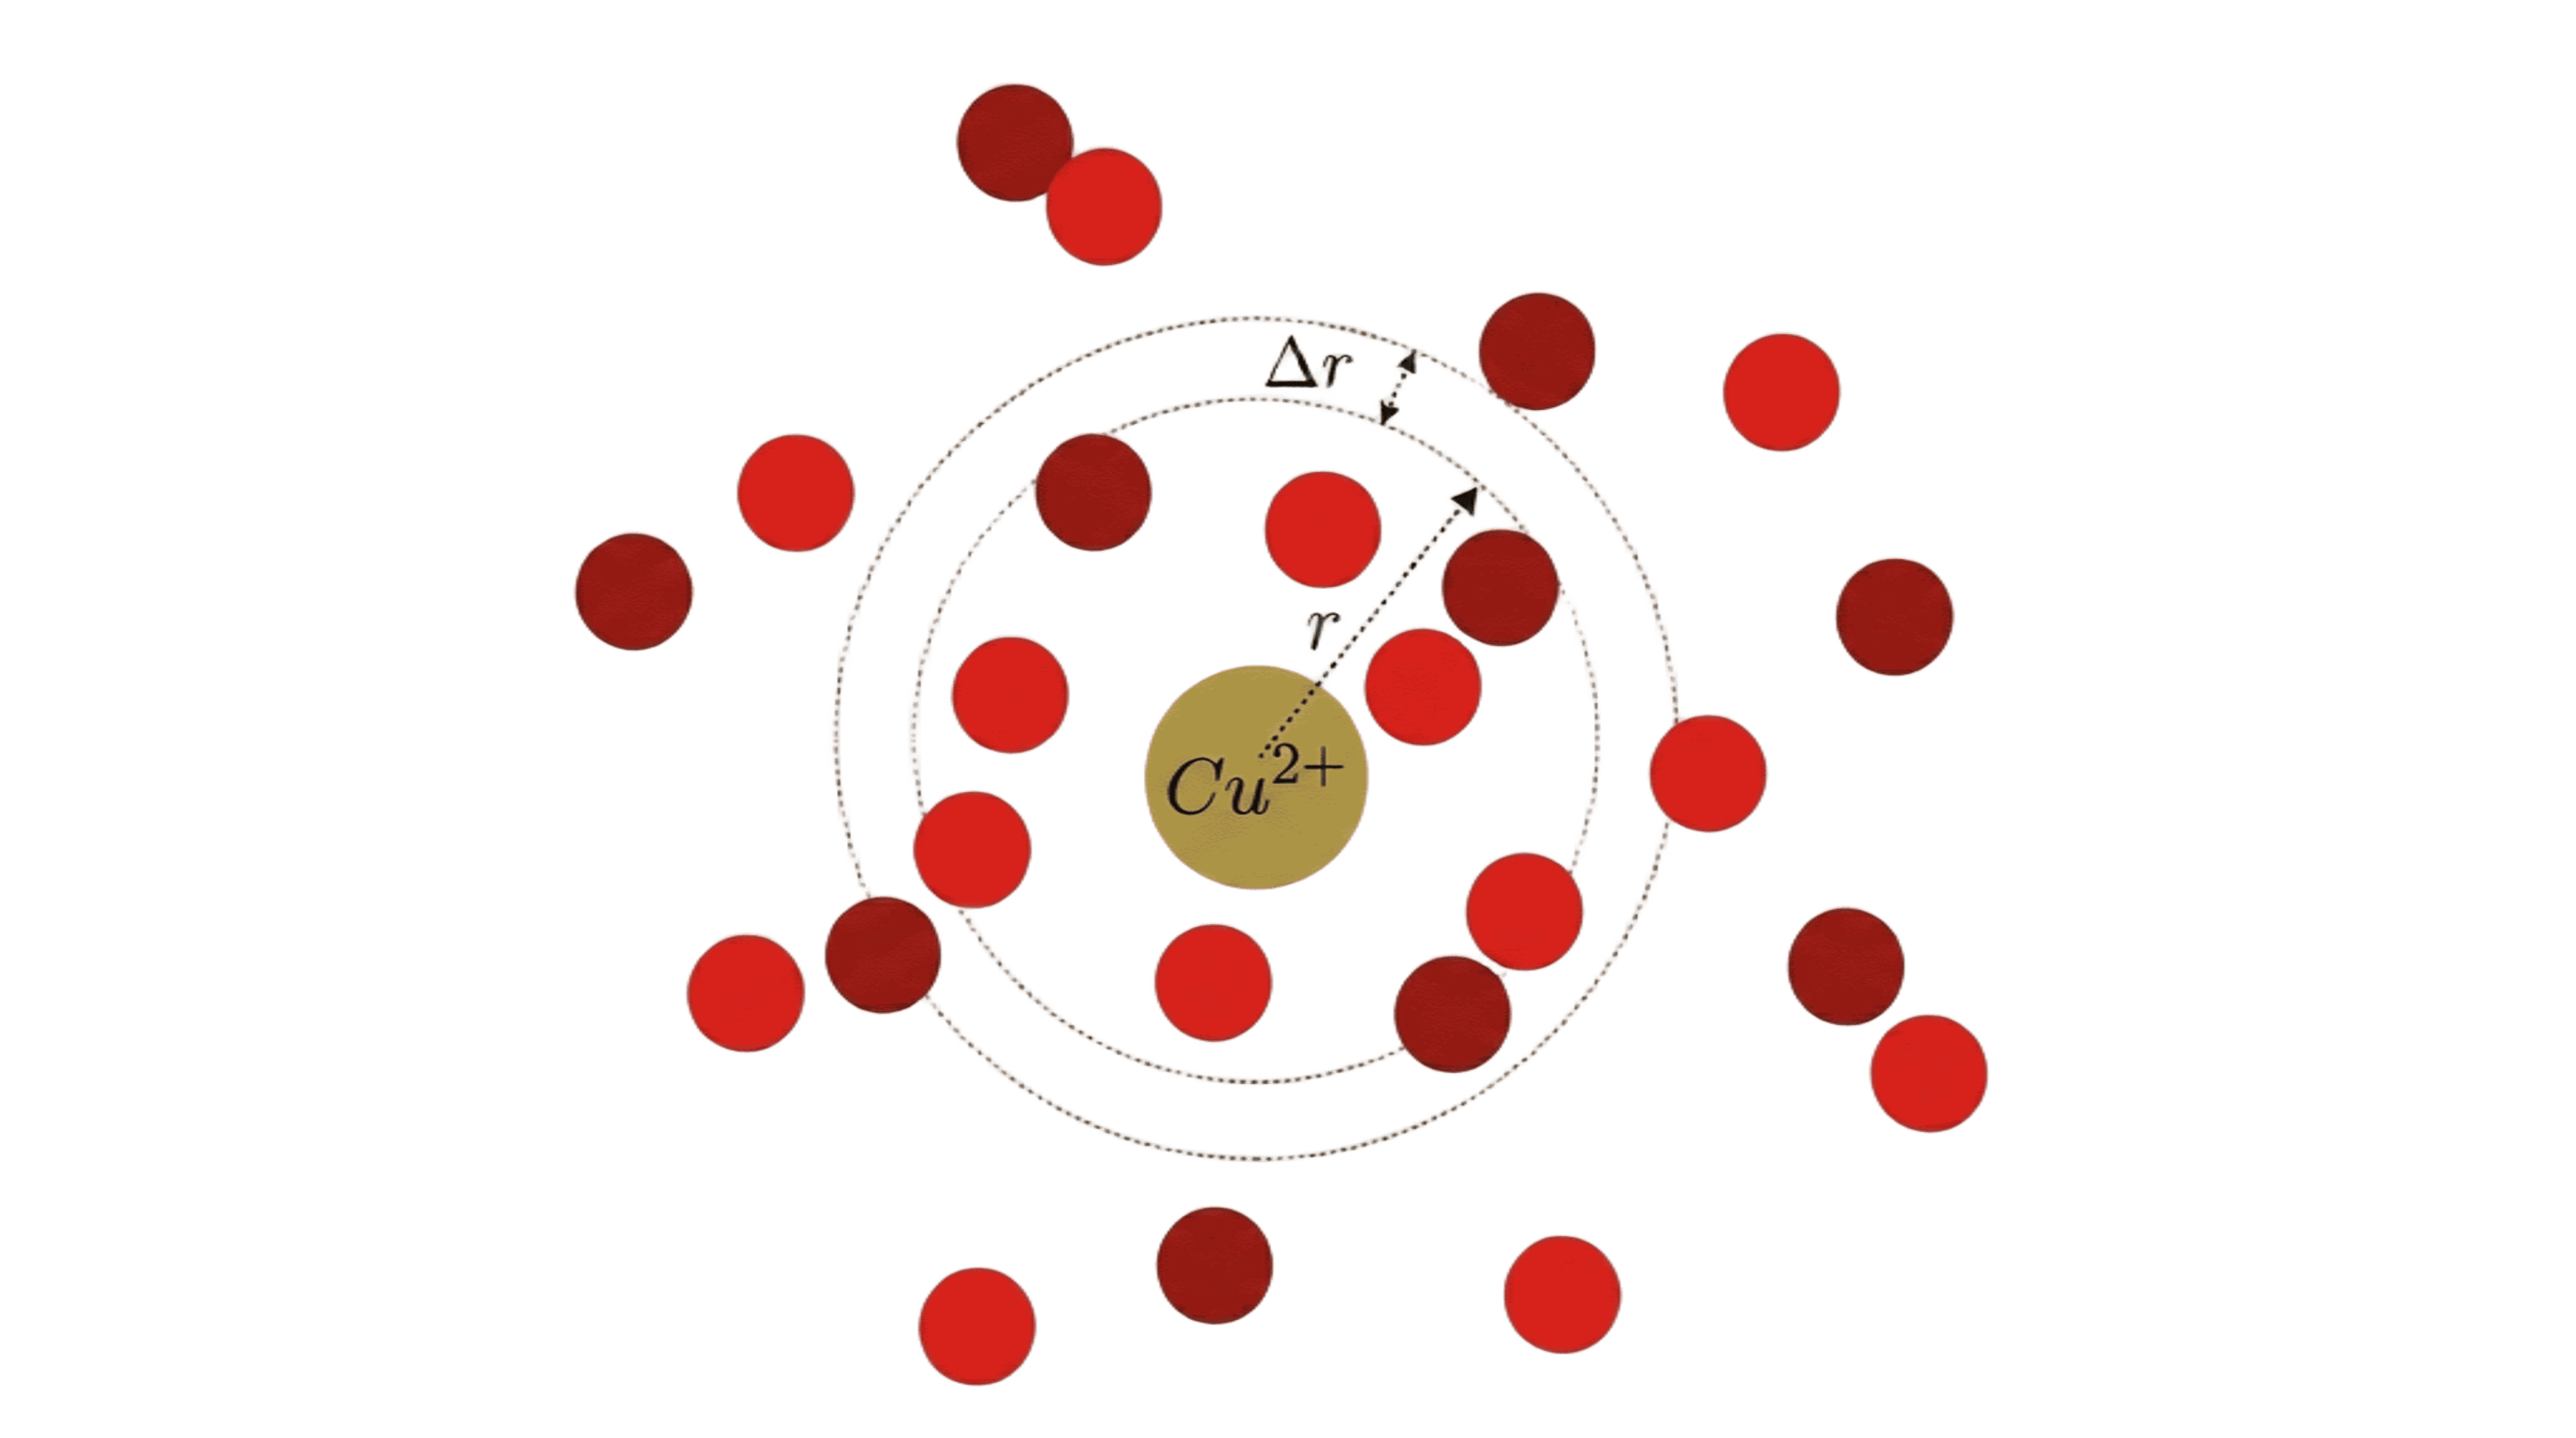
\includegraphics[width=\textwidth]{Imágenes/RDF-5.png}
    \end{minipage}
    \hfill % Espacio flexible entre las dos imágenes
    \begin{minipage}{0.38\textwidth}
        \centering
        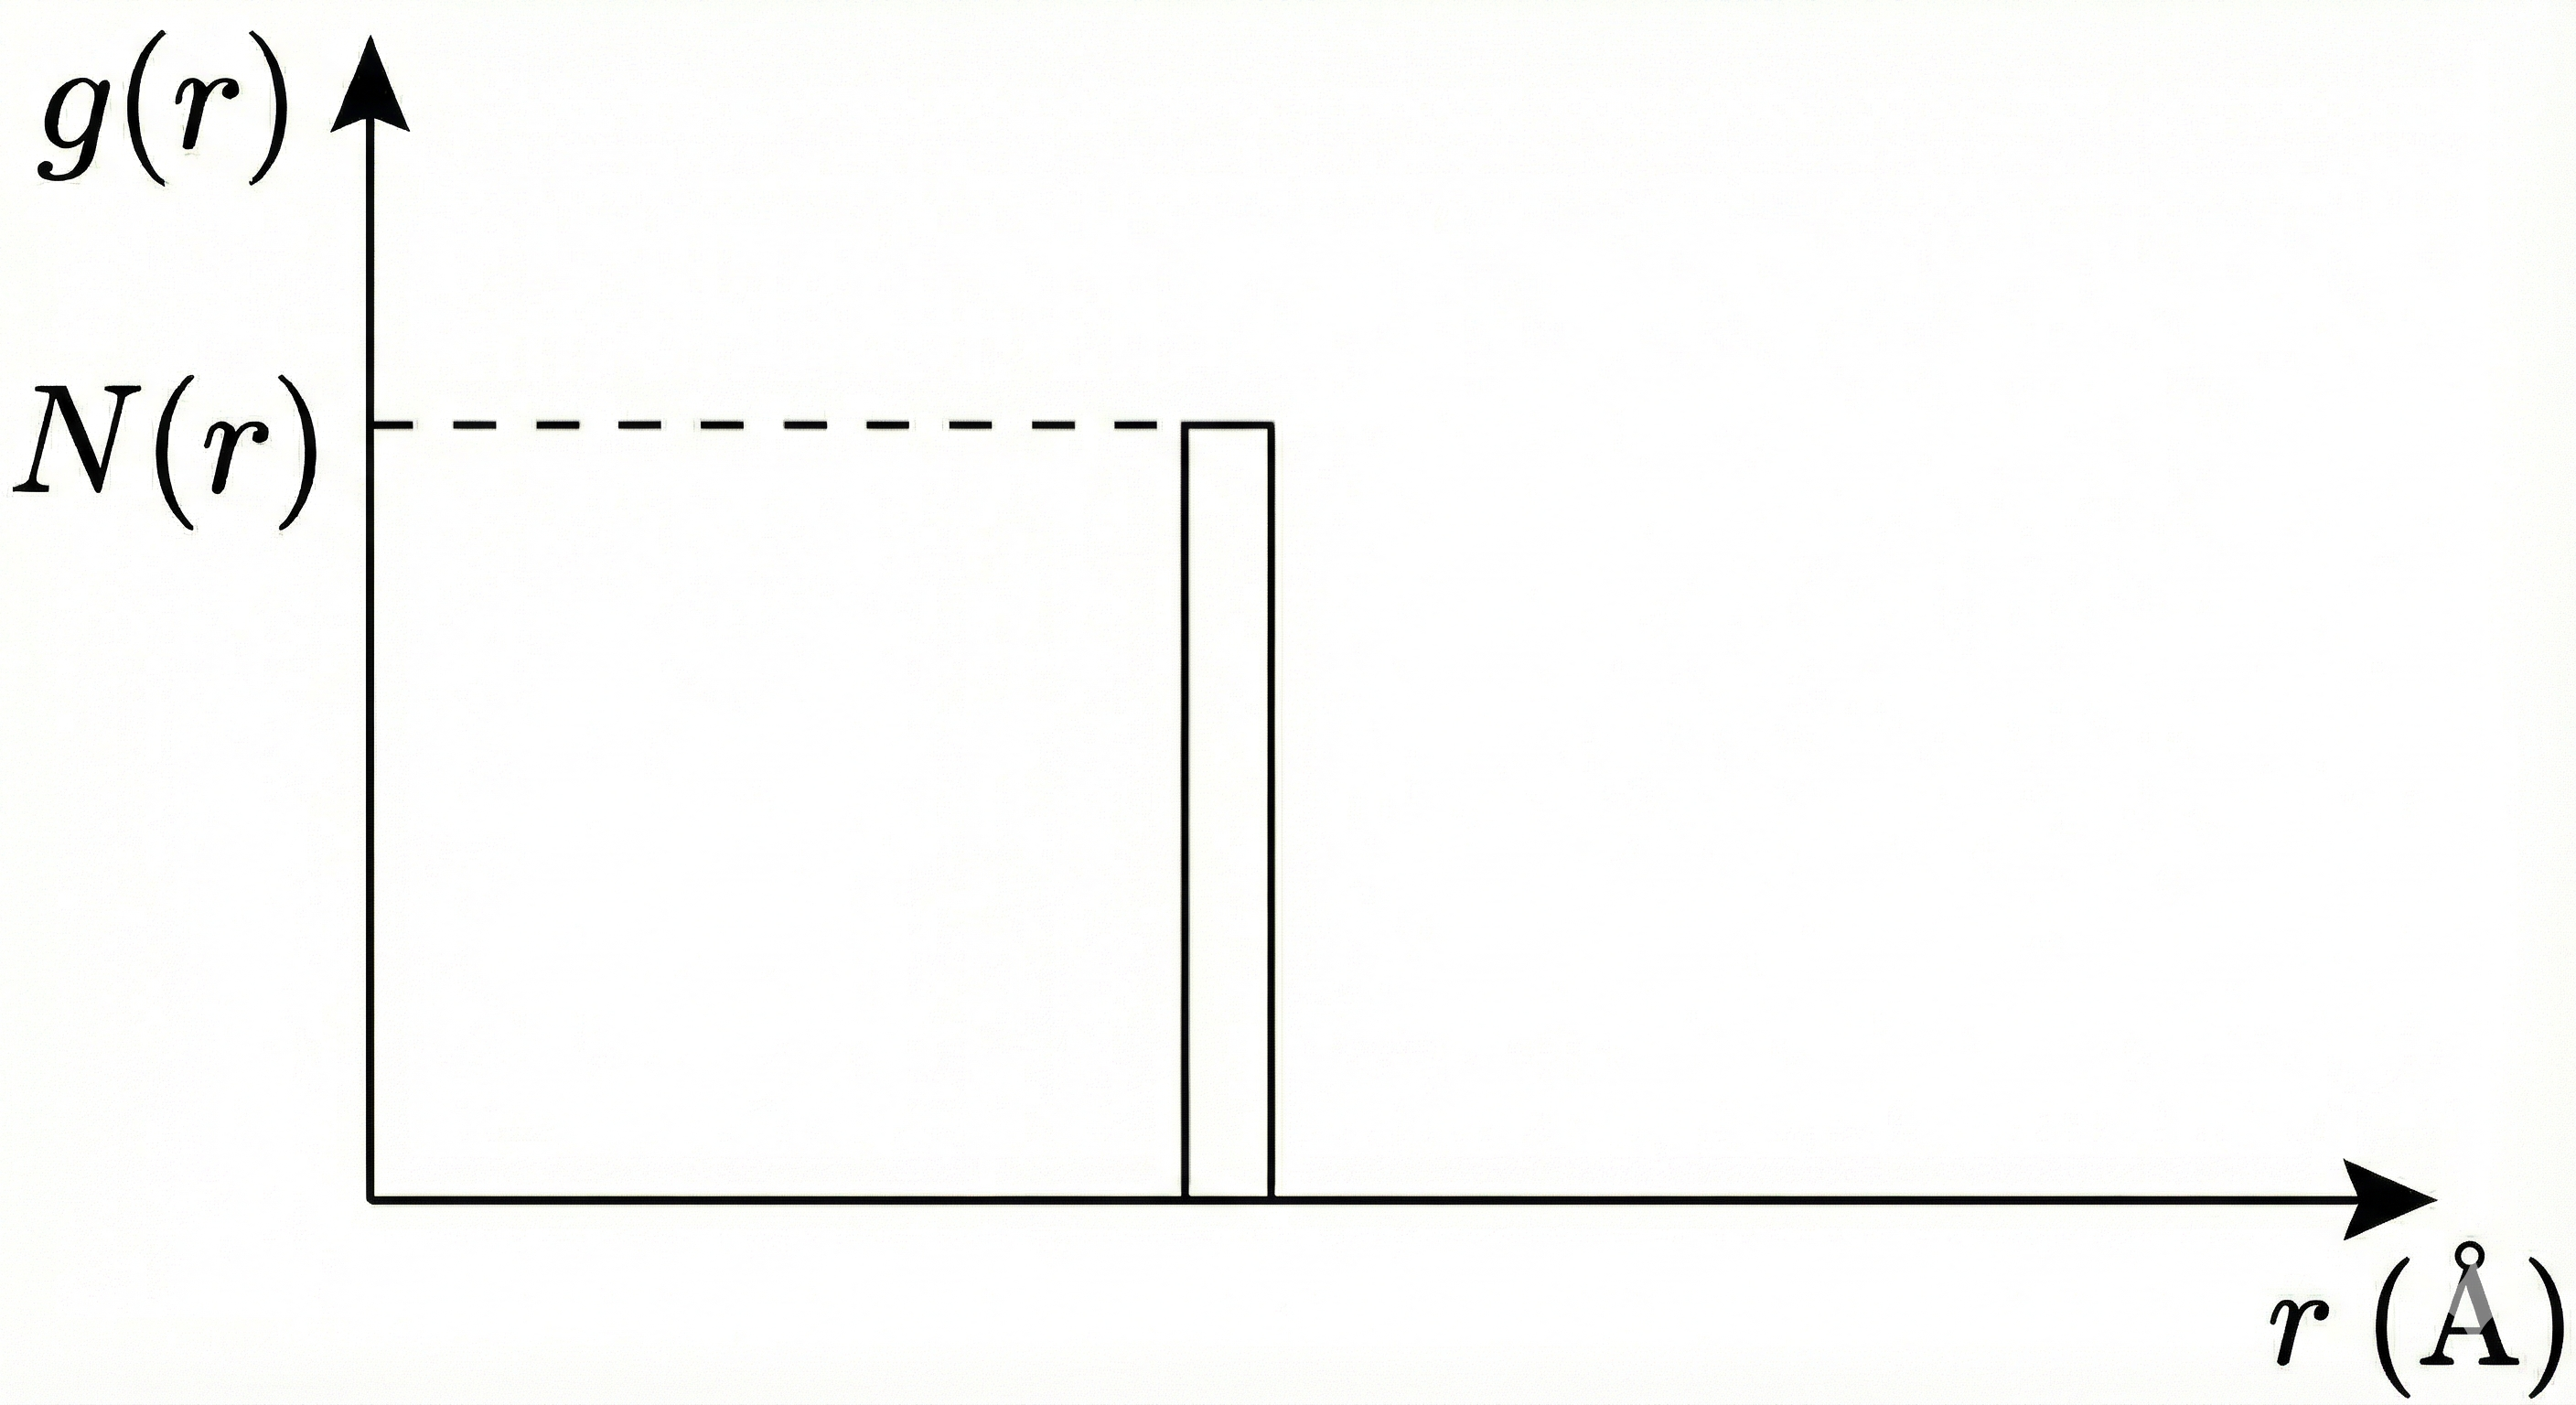
\includegraphics[width=\textwidth]{Imágenes/RDF-6.png}
       
    \end{minipage}
    \caption{Representación esquemática para el cálculo de la RDF. Se ilustra el átomo de referencia central, la distancia radial $r$ y el cascarón esférico de grosor $\Delta r$ donde se evalúa el conteo de partículas $N(r)$.}
     \label{fig:esquema_rdf}
\end{figure}

El algoritmo implementado calcula la densidad local basándose en el volumen geométrico exacto de las capas esféricas discretizadas. De esta manera, la expresión teórica general utilizada para determinar $g(r)$ en el intervalo de distancia $(r, r + \Delta r)$ queda definida como:

\begin{equation}
    g(r) = \frac{\langle N(r, \Delta r) \rangle}{\frac{4}{3}\pi \rho_{0} \left[ (r + \Delta r)^3 - r^3 \right]}
    \label{eq:rdf_general}
\end{equation}

En esta expresión, el término $\langle N(r, \Delta r) \rangle$ representa el número promedio de partículas encontradas dentro de una capa esférica de grosor $\Delta r$ a lo largo de los pasos de simulación analizados. El denominador normaliza este conteo utilizando el volumen real de dicha cáscara esférica ponderado por la densidad numérica macroscópica del disolvente, $\rho_{0}$.
%%%%%%%%%%%%%%%%%%%%%%%%%%%x

\begin{figure}[H]
    \centering
    
    % Gráfica 1 (Agua)
    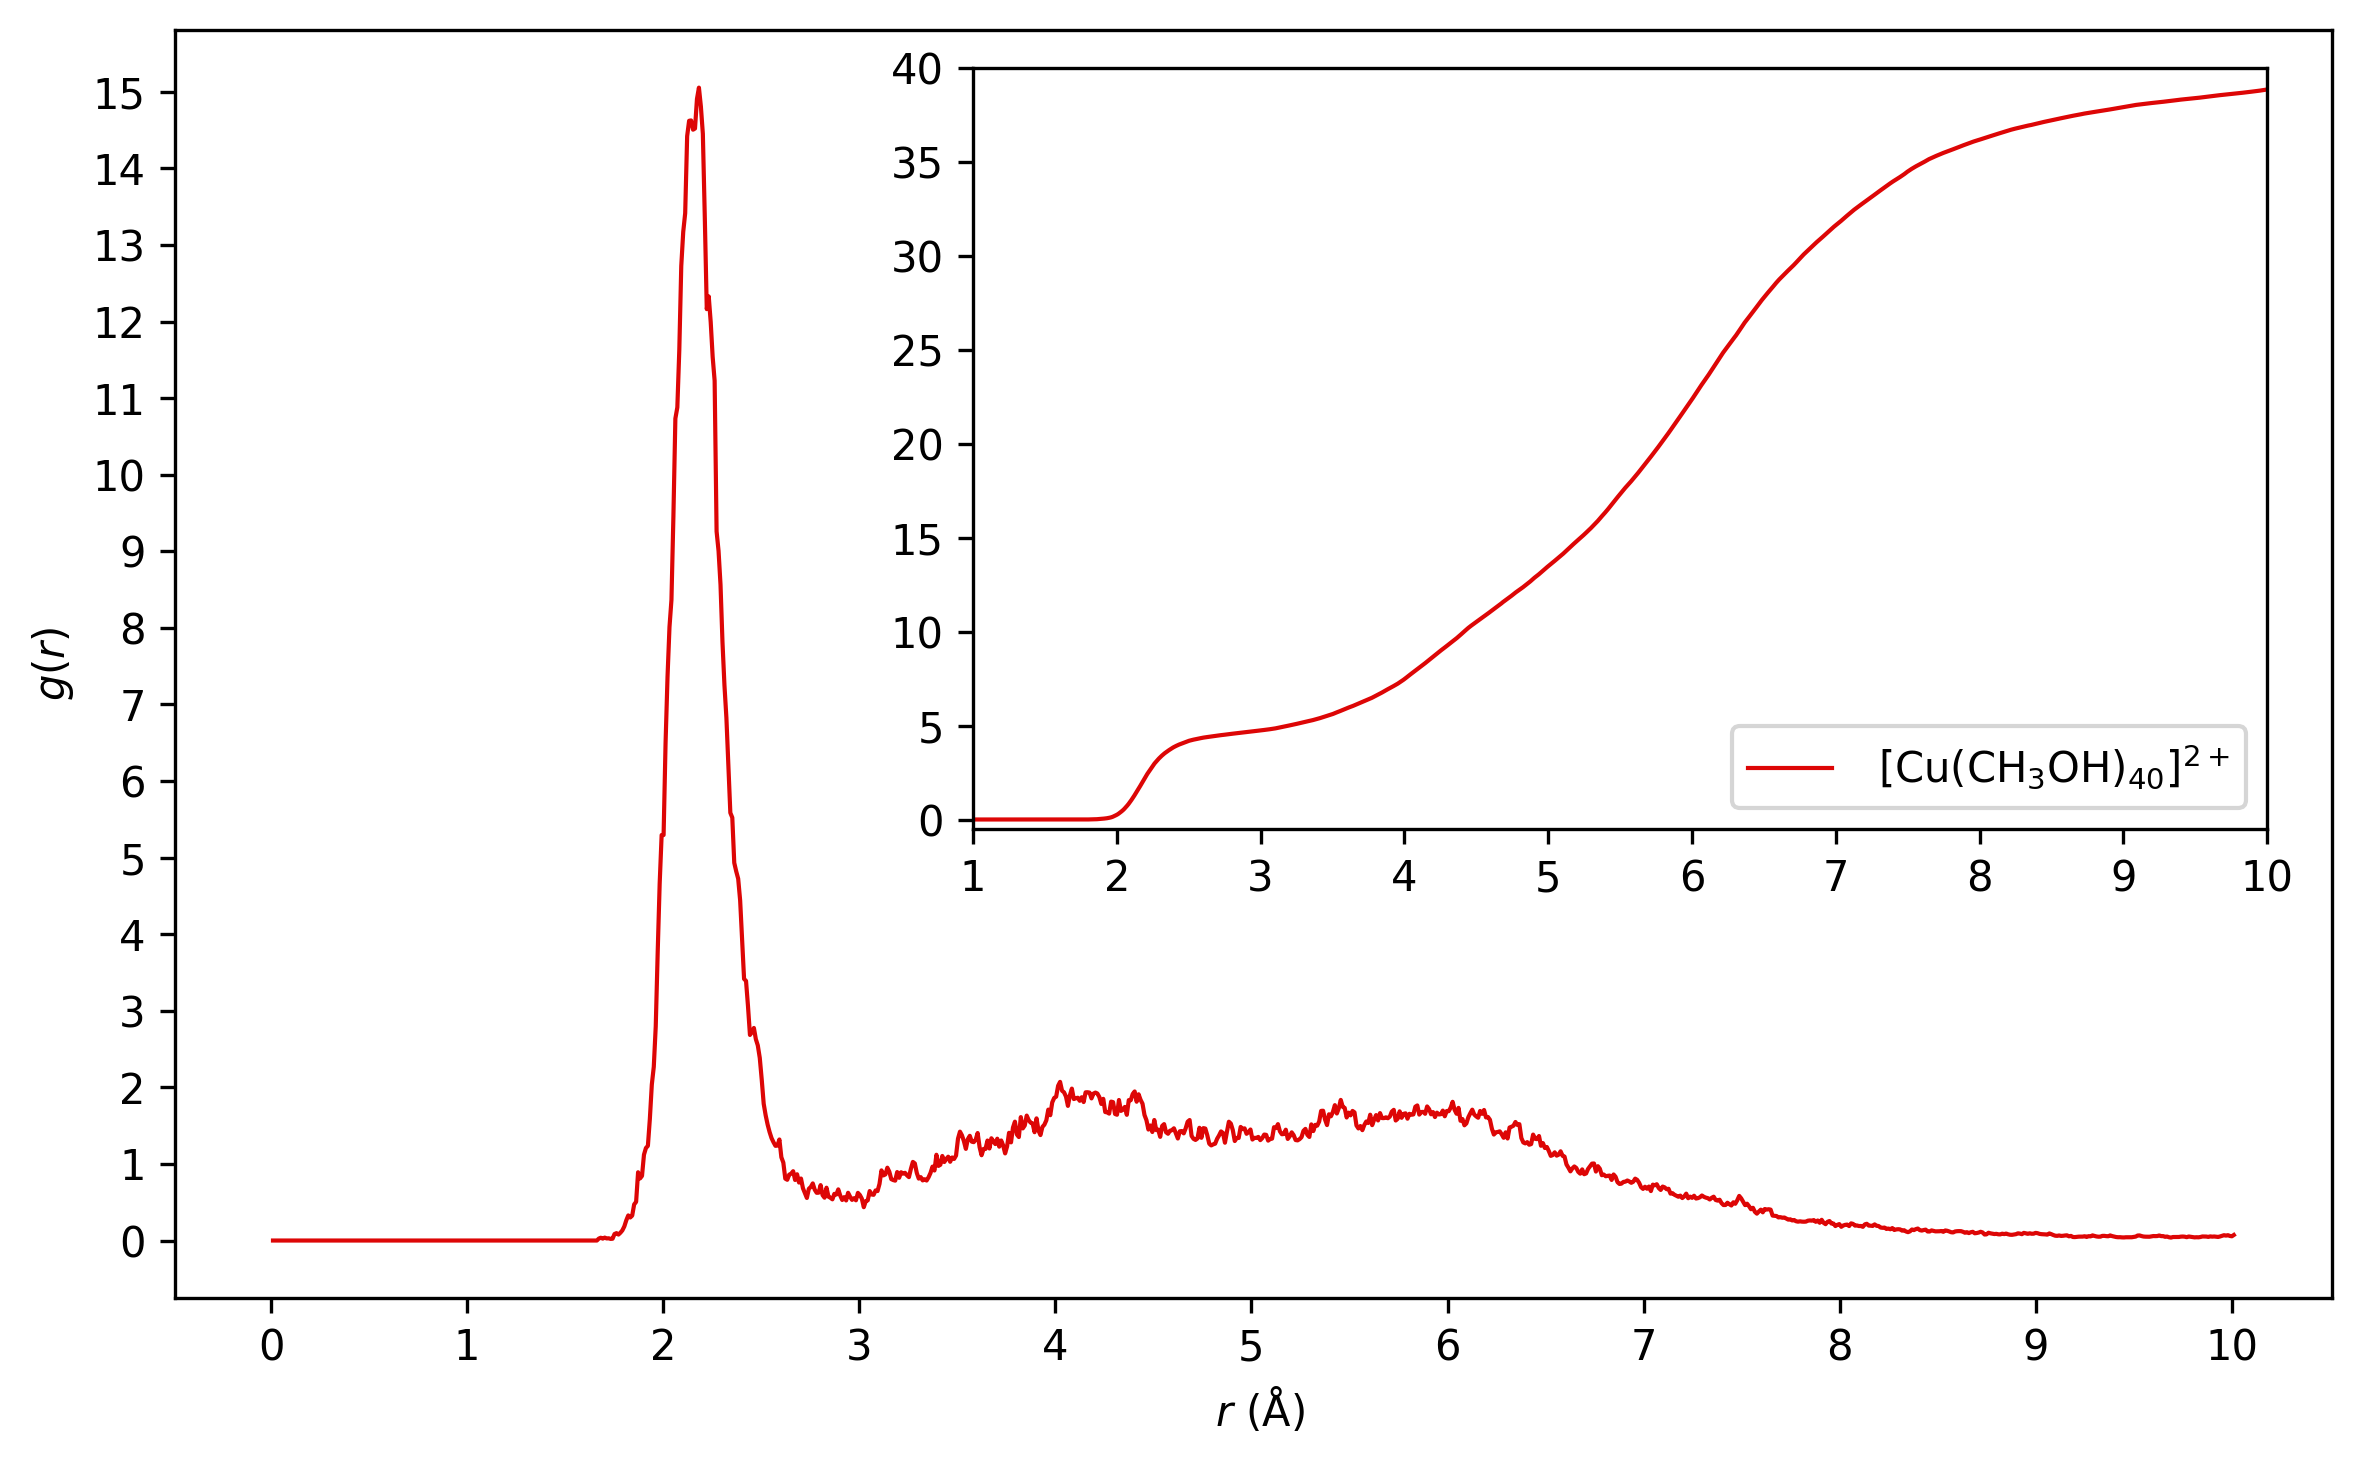
\includegraphics[width=0.85\textwidth]{Imágenes/RDF-OUTPUT-HISTOGRAMA-METANOL.png}
    
    % Un pequeño espacio vertical entre las gráficas
    \vspace{0.5cm} 
    
    % Gráfica 2 (Metanol)
    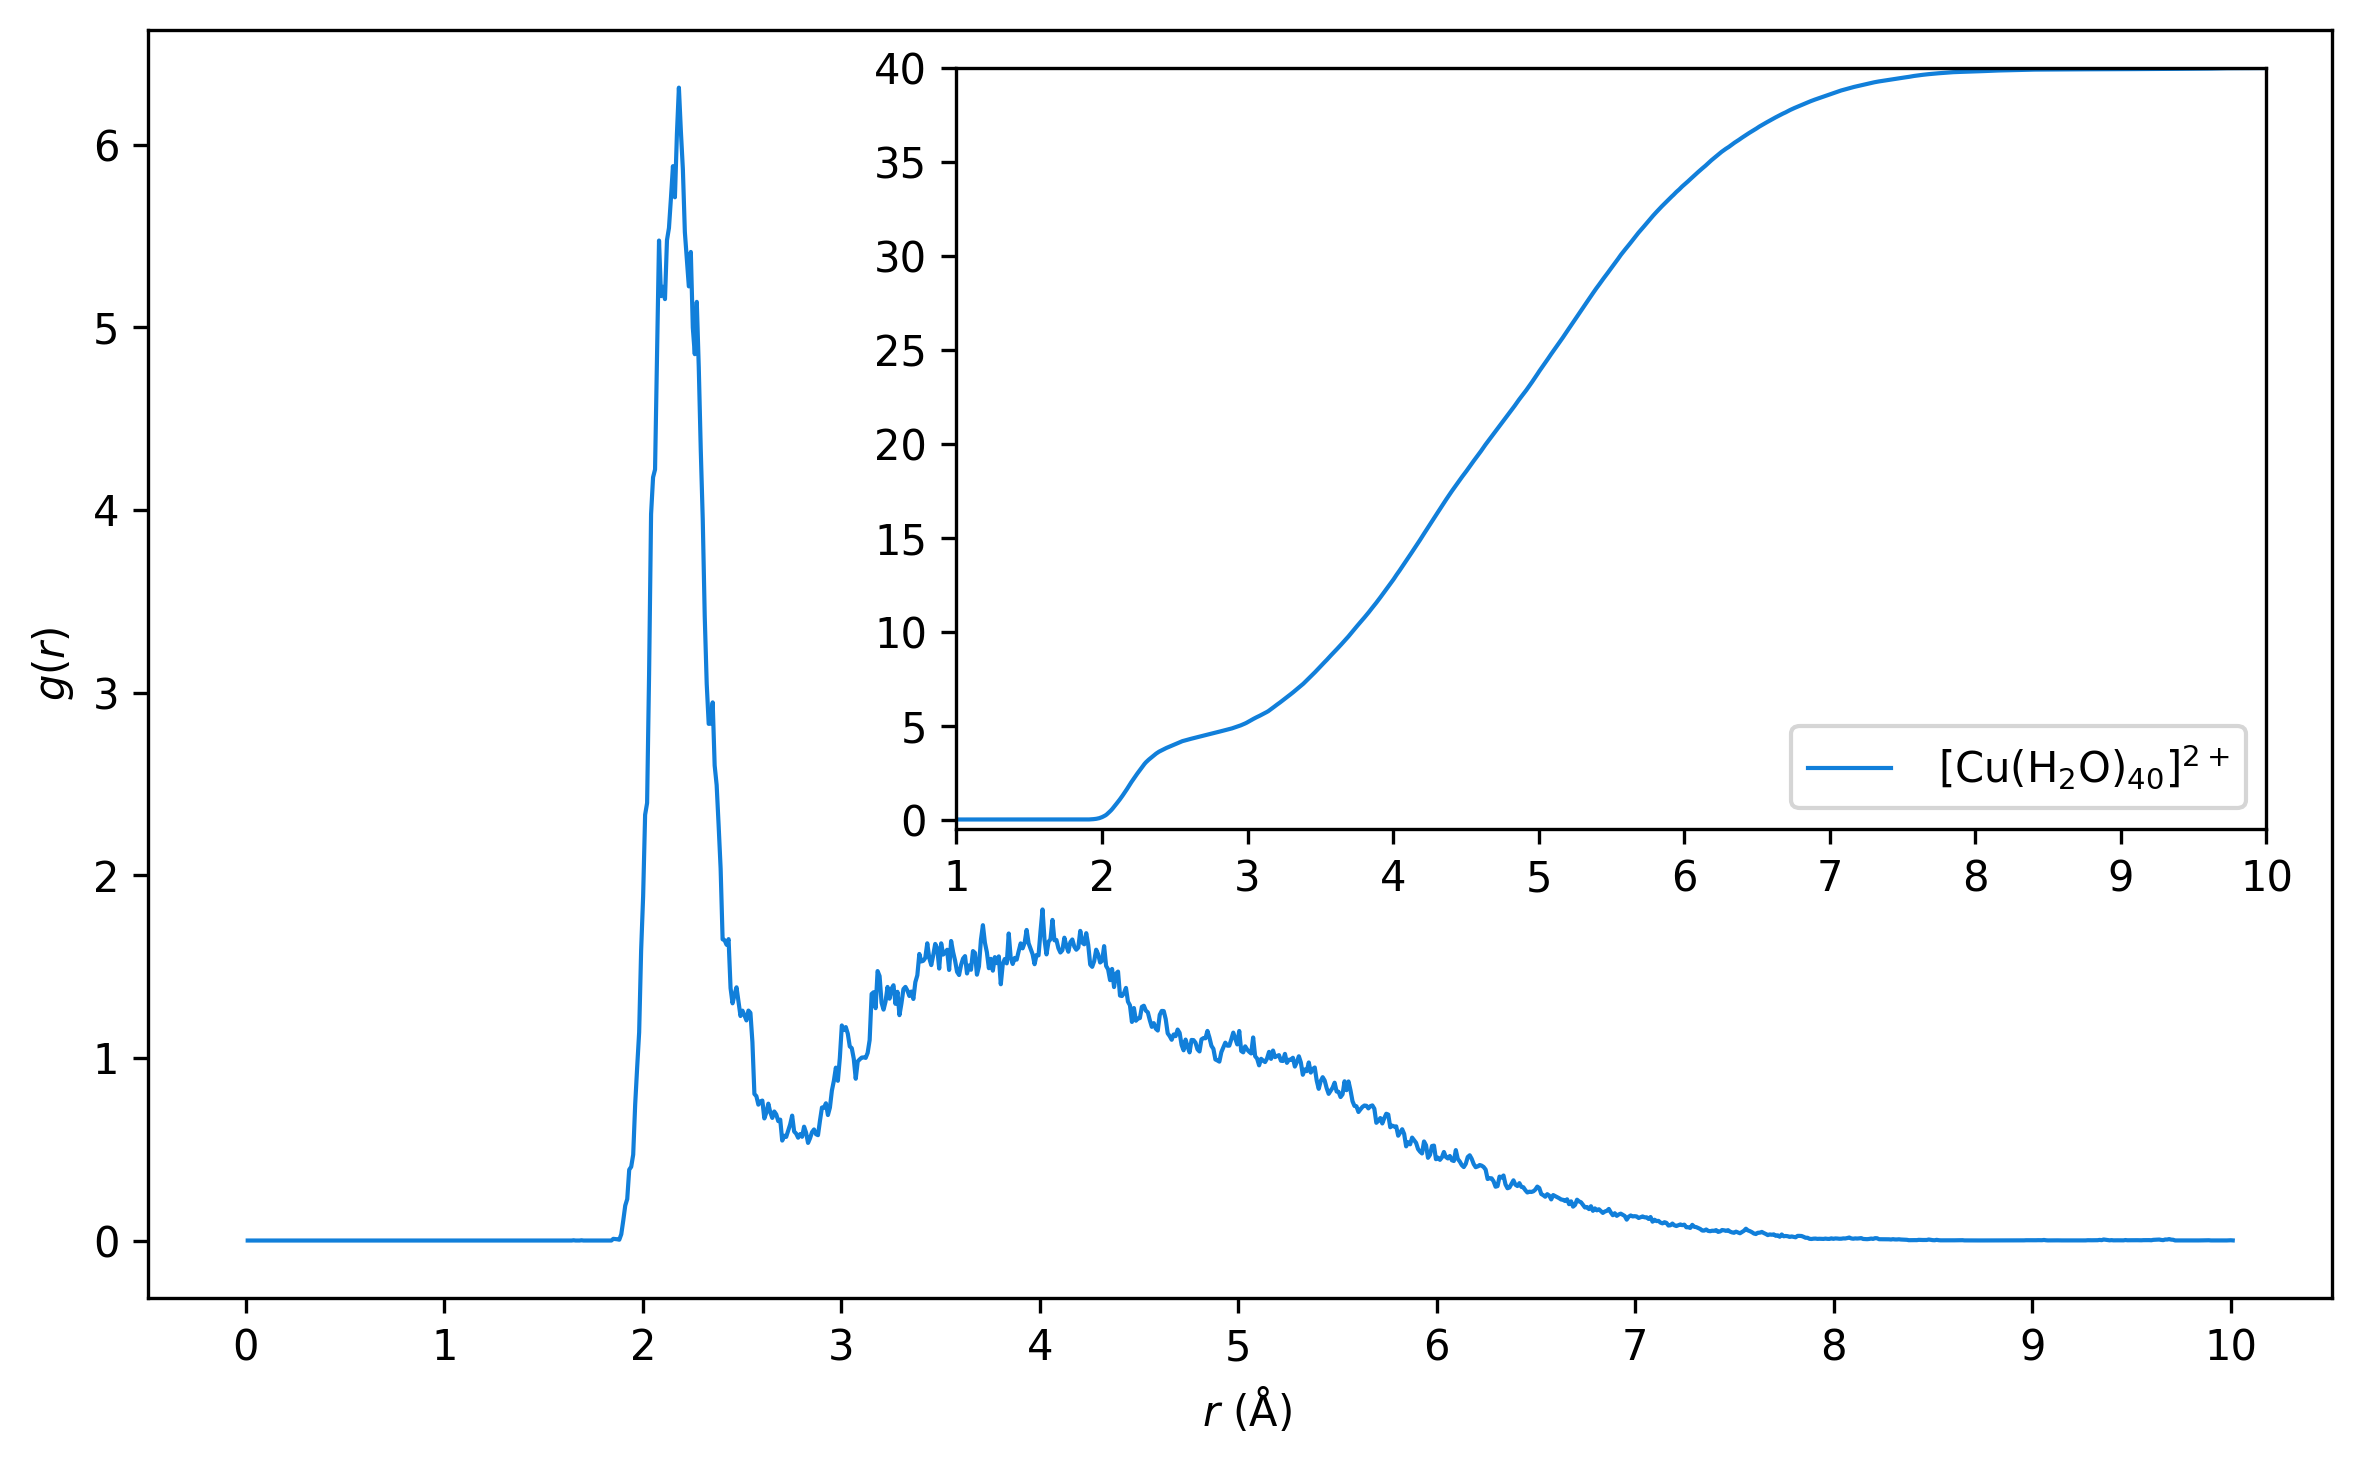
\includegraphics[width=0.85\textwidth]{Imágenes/RDF-OUTPUT-HISTOGRAMA-AGUA.png}

    % --- LEYENDA ACTUALIZADA ---
    \caption{}{Funciones de distribución radial (RDF) obtenidas para los sistemas \ce{[Cu(CH3OH)40]^{2+}} (arriba) y \ce{[Cu(H2O)40]^{2+}} (abajo) a partir de las simulaciones de dinámica molecular.}
    \label{fig:bases2}
\end{figure}


\section{Función de Distribución Angular}
